\chapter{Venting and Bakeout}
\section{Venting}
Ion pump and ion pressure gauge should be off well in advance (day before for ion pump, few hours for ion gauge) of venting because when they are on, they contain hot filaments which could oxidize when exposed to air.
\begin{enumerate}
\item	If not already done so, flush the water cooling lines (see flushing procedure) turn off chiller and remove the cooling lines from evaporator(s) that are removing.
\item	Retract the crystal thickness monitor rod to the marked position.
\item	Vent the system. (Keep gate valve open).
\begin{enumerate}
\item	Run turbo pump overnight before venting? Why do you need to pump system down when goal is to bring to atmosphere?
\item	Make sure ion gauge is off: when it’s off, the left display (MBE system pressure) will not display a reading. If it is not off, need to turn it off and wait a few hours for filament to cool down before venting.
\item	Venting is done with in-house N2 since we do not want fill the MBE with air. Open the N2 valve behind the AFM desk and to the left of the compressed air valve. Make sure to use N2 and not compressed air! Open the valve at end of N2 pipe (white) and adjust the regulator until feel proper N2 pressure: want a gentle N2 flow since venting slowly is safer. Insert the N2 pipe into black pipe which comes out of turbo pump.
\item	On touch screen press: \emph{turbo pump} $\rightarrow$ \emph{vent} $\rightarrow$ \emph{yes}. This turns off both roughing and turbo pump. Turbo takes some time to slow down. The system will gradually fill with N2 and can hear the soft air flow sound going in through the turbo. Need to wait until the soft noise is almost gone which means the system is vented. The small pressure reading in right display reads it near the turbo pump, so it doesn’t indicate pressure inside MBE. It can be used for rough estimate of if pressure is rising or falling. When the air flow sound disappeared, pressure showed 2.8e0mB. The flexibility of the bevel on the manipulator can also help determine if system has been vented enough.
\end{enumerate}
\end{enumerate}

\section{Removing evaporators}
\begin{enumerate}
\item	Need 2 people for this. Wearing clean gloves, use 2 wrenches (size10) to unscrew the nuts that hold the evaporator in place. When removing last nuts, one person needs to hold the evaporator. Very carefully pull the evaporator straight out of the system (it is quite long and need to not hit any part of it against system). Make sure to not hit the wobble stick when standing up! \\\\
For the W evaporator, its source is a rod so can carefully put the metal protective tube/shield onto evaporator (1 person should hold evaporator steady), making sure to not hit components against the shield, and use the nuts the hold it in place. Wrap around near evaporator-shield connection point with large Kimwipes and then foil. Then can lay the W evaporator down, supporting it on the shutter and electrical connection "legs". \textbf{If the Sn evaporator has source in it, can never lay it down!}. Once person must always hold it upright until the source crucible is removed.
\item	After have placed shielded evaporator in safe and stable location, need to cover the evaporator opening in MBE system using a flange.  First wipe it with IPA and then put a new Cu gasket into the slot. 
\item	Attach the cover with the same nuts used for evaporator to the opening. For tightening components on vacuum systems need to ensure that do it evenly. Here dealing with small components so it is not so strict. Must make sure that you are always turning in the correct direction (tightening and not loosening) because if loosen after tightening and then tighten again, this could result in leakage. Correct direction for tightening is clockwise when looking at the nut or bolt from the side that’s facing out. First hand-tighten all the nuts. Then go in a crisscross pattern and tighten about $1/4$ turn. Then go around in circles, gradually tightening each nut about the same amount. Do not apply too much force when tightening. Due to space limitations, it seems easier to hold the bolt in place while tightening the nuts from the bottom. Make sure to not hit the wobble stick which will be right above your head!
\item	 After the cover(s) are on, need to pump down the system. It is not good to leave the system at atmosphere pressure even though is filled with N2. To pump down:
\begin{enumerate}
\item	Turn off N2 flow but don’t disconnect the tube from turbo pump, otherwise it lets air into pump which could make it harder to pump. 
\item	Turn on turbo pump. Will at first hear a loud noise of the roughing pump motor. This noise seems louder than when turn on turbo pump on a system already at vacuum but is probably because of the higher pressure difference/more work the pump needs to do when pumping from atmosphere. The turbo will turn on and speed up automatically until it reaches max speed. 
\item	After ~1hr pumping, can turn on ion gauge: At top control buttons press the book button, then display will say “emission auto?” then press checkmark button. Right display pressure reading was 5.8e-1 at this time. MBE pressure (left display) was 1.2e-6. MBE pressure dropped to ~5e-7 about 2hrs after started pumping.
\end{enumerate}
\end{enumerate}


\section{Bakeout}
Must follow all steps carefully!
\begin{enumerate}
\item Make sure maintenance work on evaporators is completed and source materials installed. Make sure a clean blank sample holder is in FEL, no sample plate in MBE heater stage.
\item	Start pumping down MBE+FEL by turning on turbo pump. Keep ion pump off. Gate valve [MBE chamber, FEL] is open, metal valve [Turbo molecular pump, FEL] is closed. System needs to reach good vacuum before start baking.
\item	Thoroughly flush water cooling lines with air. Increase air pressure by $1/2$ turn at valve behind AFM computer. Remember to decrease it back when done. Must flush significantly longer $>30$min each line) than for regular shut-down of water chiller since water vapor in lines during bakeout can cause damage.
\item	Disconnect water cooling lines including the thicker lines above the T-shaped connectors with valves (these lines need to be slit with knife to be able to remove them). 
\item	Disconnect evaporator electronic connections. For safety, unplug corresponding power supplies before removing Se evaporator cable connections. 
\item	Use IPA to clean the chamber surfaces and viewports.
\item	Move thickness monitor in to avoid it being hit by bakeout panel. For bakeout need to move in the protrusion so the bakeout wall doesn’t hit it. The middle sharpie mark is bakeout. We don’t move it all the way in because that put unnecessary (in the sense that the moving in part of the way already ensures that it doesn’t hit the bakeout wall) stress on the bevel right above the thing we are turning (bevel gets compressed a lot).
\item	Cover viewports with 3 layers of foil to protect during bakeout.
\item	Remove the plastic handle for metal valve [Turbo, FEL].
\item   Remove the black magnetic couplers from transfer arms. Since there is high risk of the FEL transfer arm to jump when remove coupler and therefore for the blank (recall that we install a blank onto the transfer arm in FEL before bakeout, so that after bakeout can easily transfer it into MBE for degassing. Recall that for degassing things need a blank on the heater stage to protect it.), it is not good idea to first pump down FEL, and then try to remove coupler (we did it this way before). If blank falls, then need to vent FEL, reinstall blank again and then it might fall again.\\
Way to do it:
\begin{enumerate}
\item	Vent FEL together with the MBE by having [MBE,FEL] valve open, but [FEL, turbo] metal valve closed (since want there to be only 1 pathway for venting (through the gate valve (touchscreen controlled).  
\item	Open FEL viewport and install blank to transfer arm (make sure that have already taken out any samples/sample plates from the heater stage!). 
\item	Gently close viewport using same gasket and just few nuts (this is so that if blank falls while taking off the coupler, it does not fall out of viewport). 
\item	Now slowly remove the coupler. If blank falls, it’s not a big issue, just open viewport again and reinstall blank and try again.
\item	Once ready to pump down MBE, pump it down along with FEL, by keeping the valves in the configuration described above.
\end{enumerate}
\item	Make final checks before install bakeout panels: 
a.	Make sure no stray objects are lying on the system and all viewports are covered with foil.
b.	Valves are in correct position.
c.	All electrical wires that need to be removed are removed (LEDs, evaporator connections etc)
d.	Evaporator shutters are closed.
\item	Install baking panels (see installation order below) and 2 heating blankets (for transfer arm and linear transfer line to STM). Connect power for the heating blankets.
\subsubsection*{Panels setup}

\begin{figure}[H]	\vfill
	\begin{minipage}[c]{0.33\linewidth}  %TO GET PORTRAIT AND LANDSCAPE MODE IMAGES TO BE ON SAME LINE USE [c] FOR THE ALIGNMENT OF MINIPAGES NOT [b]!!!!
		\centering
		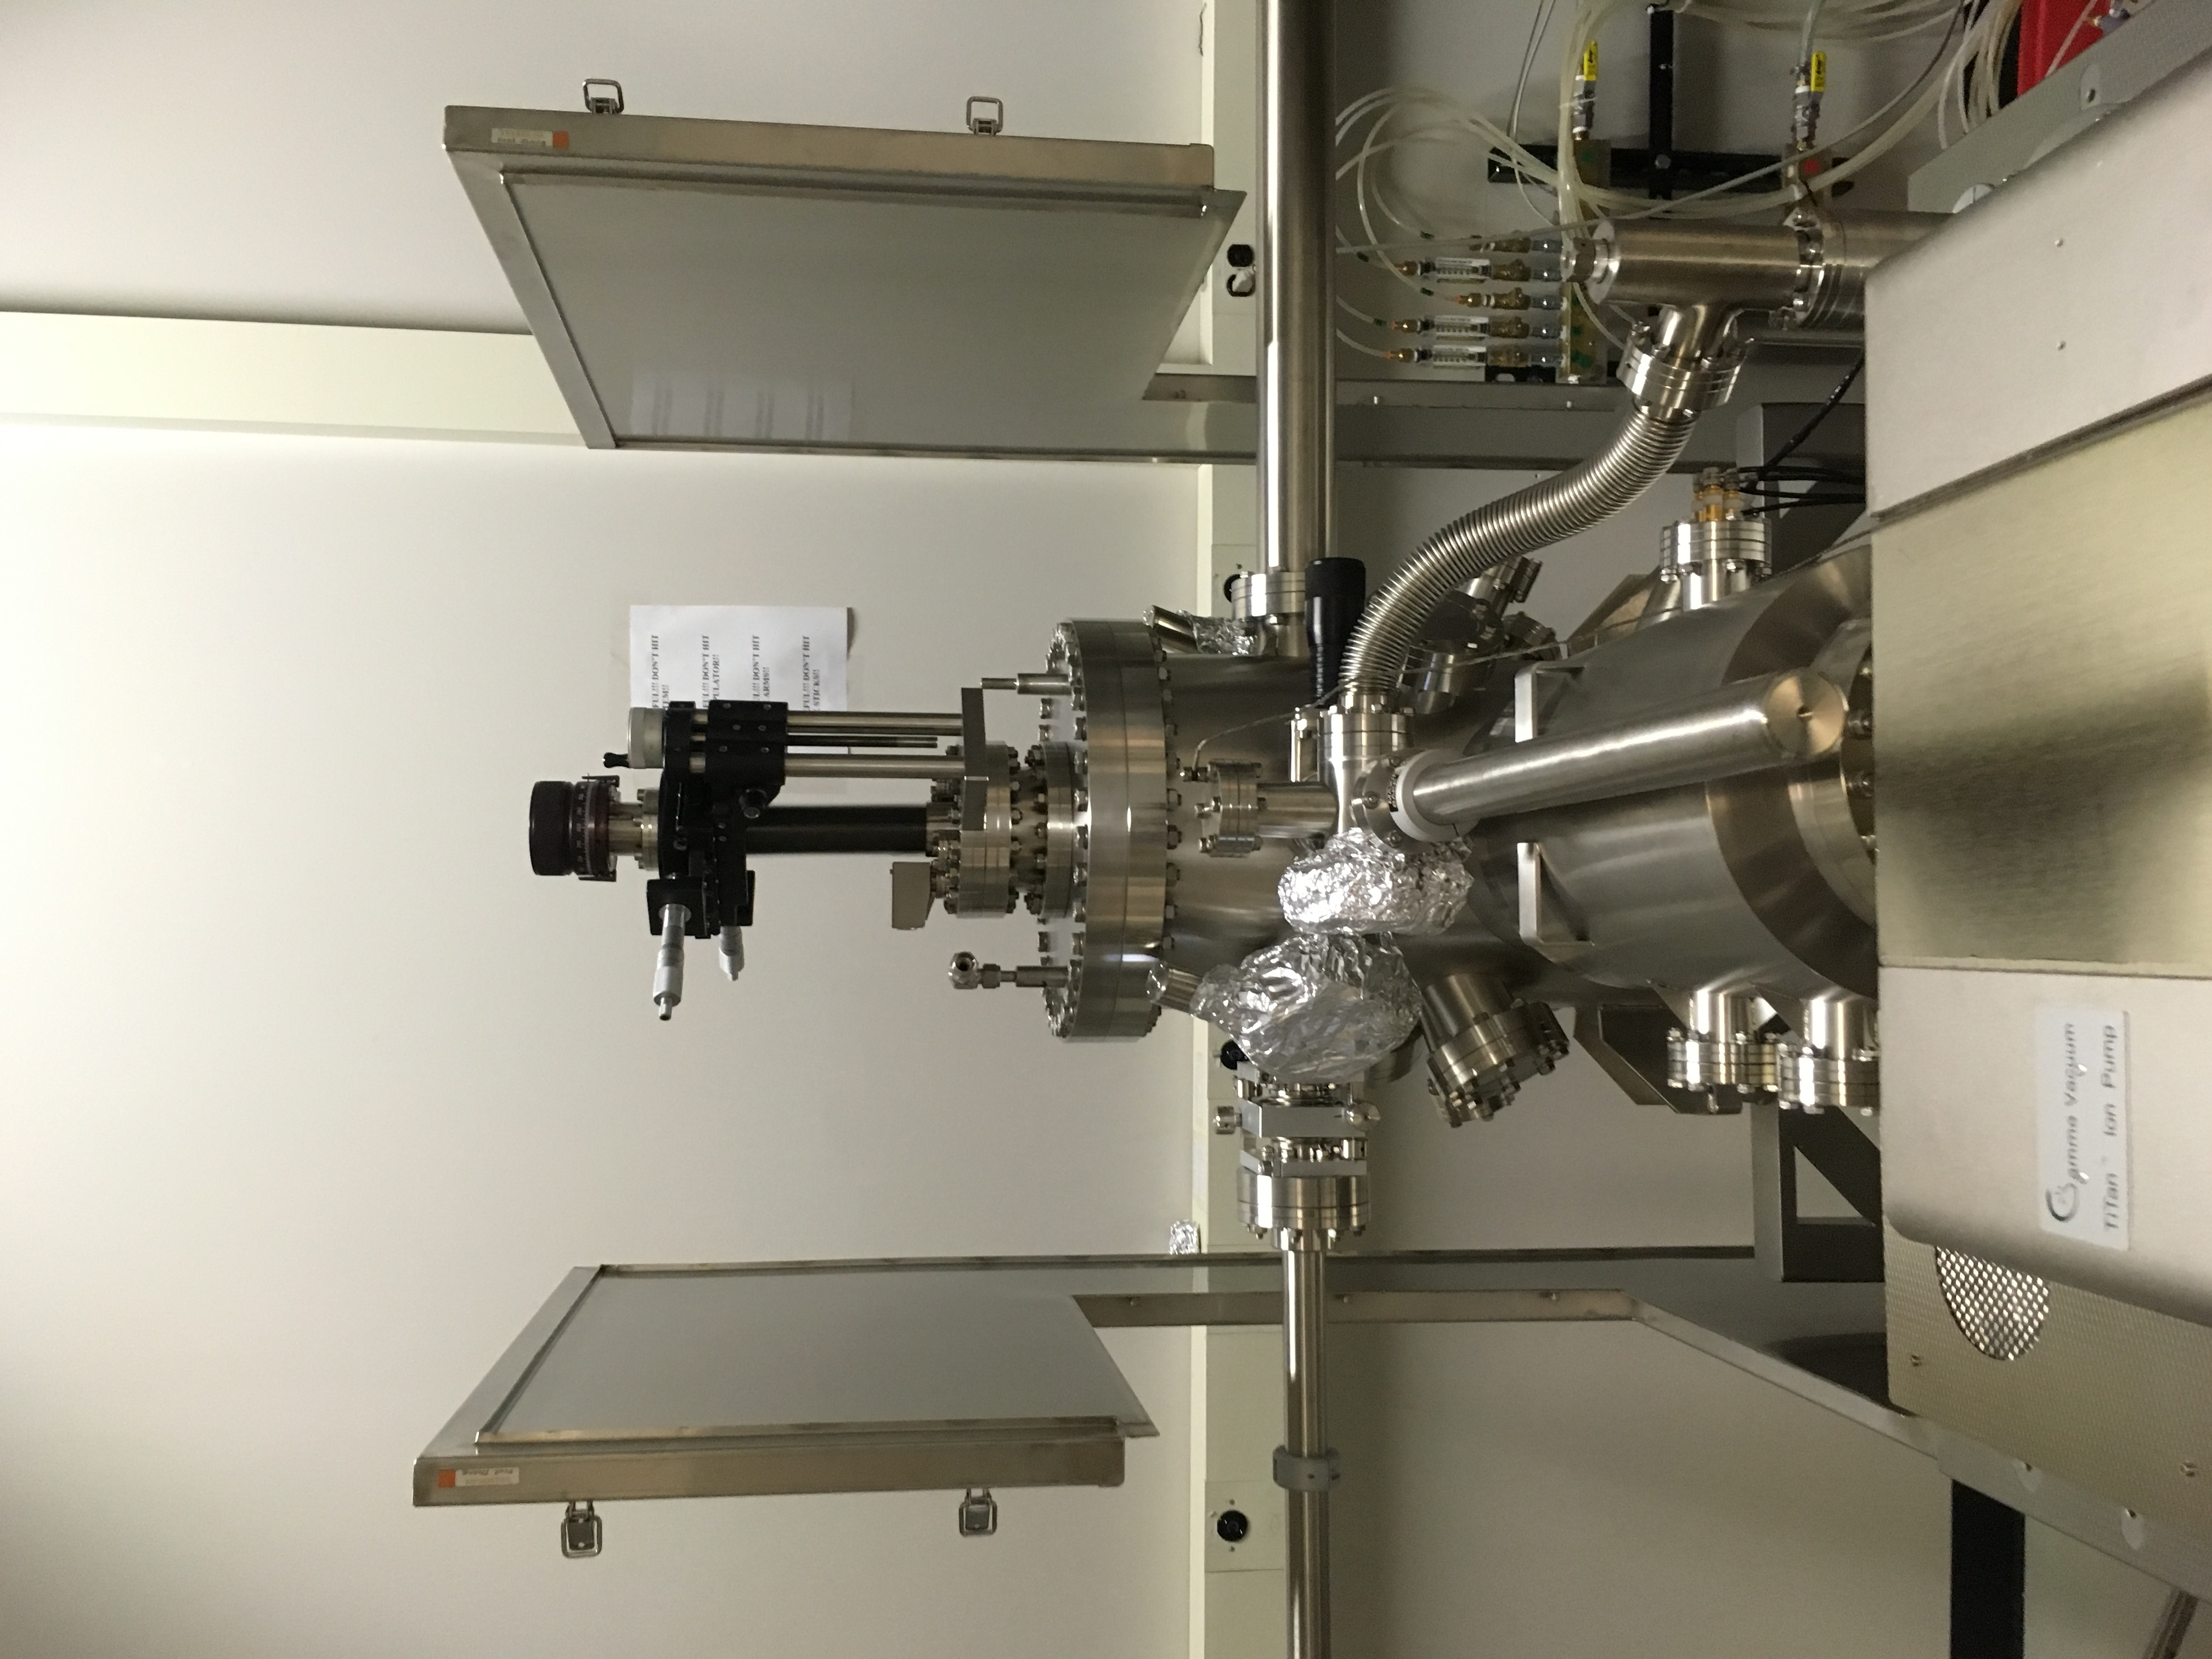
\includegraphics[width=1\textwidth, angle=270]{panels1.jpg} %NEED TO ROTATE SOME OF THESE BECAUSE LATEX IS DISPLAYING THEM  WRONG!: USE angle =  for that.
	\end{minipage}\hfill
	\begin{minipage}[c]{0.33\linewidth}
		\centering
		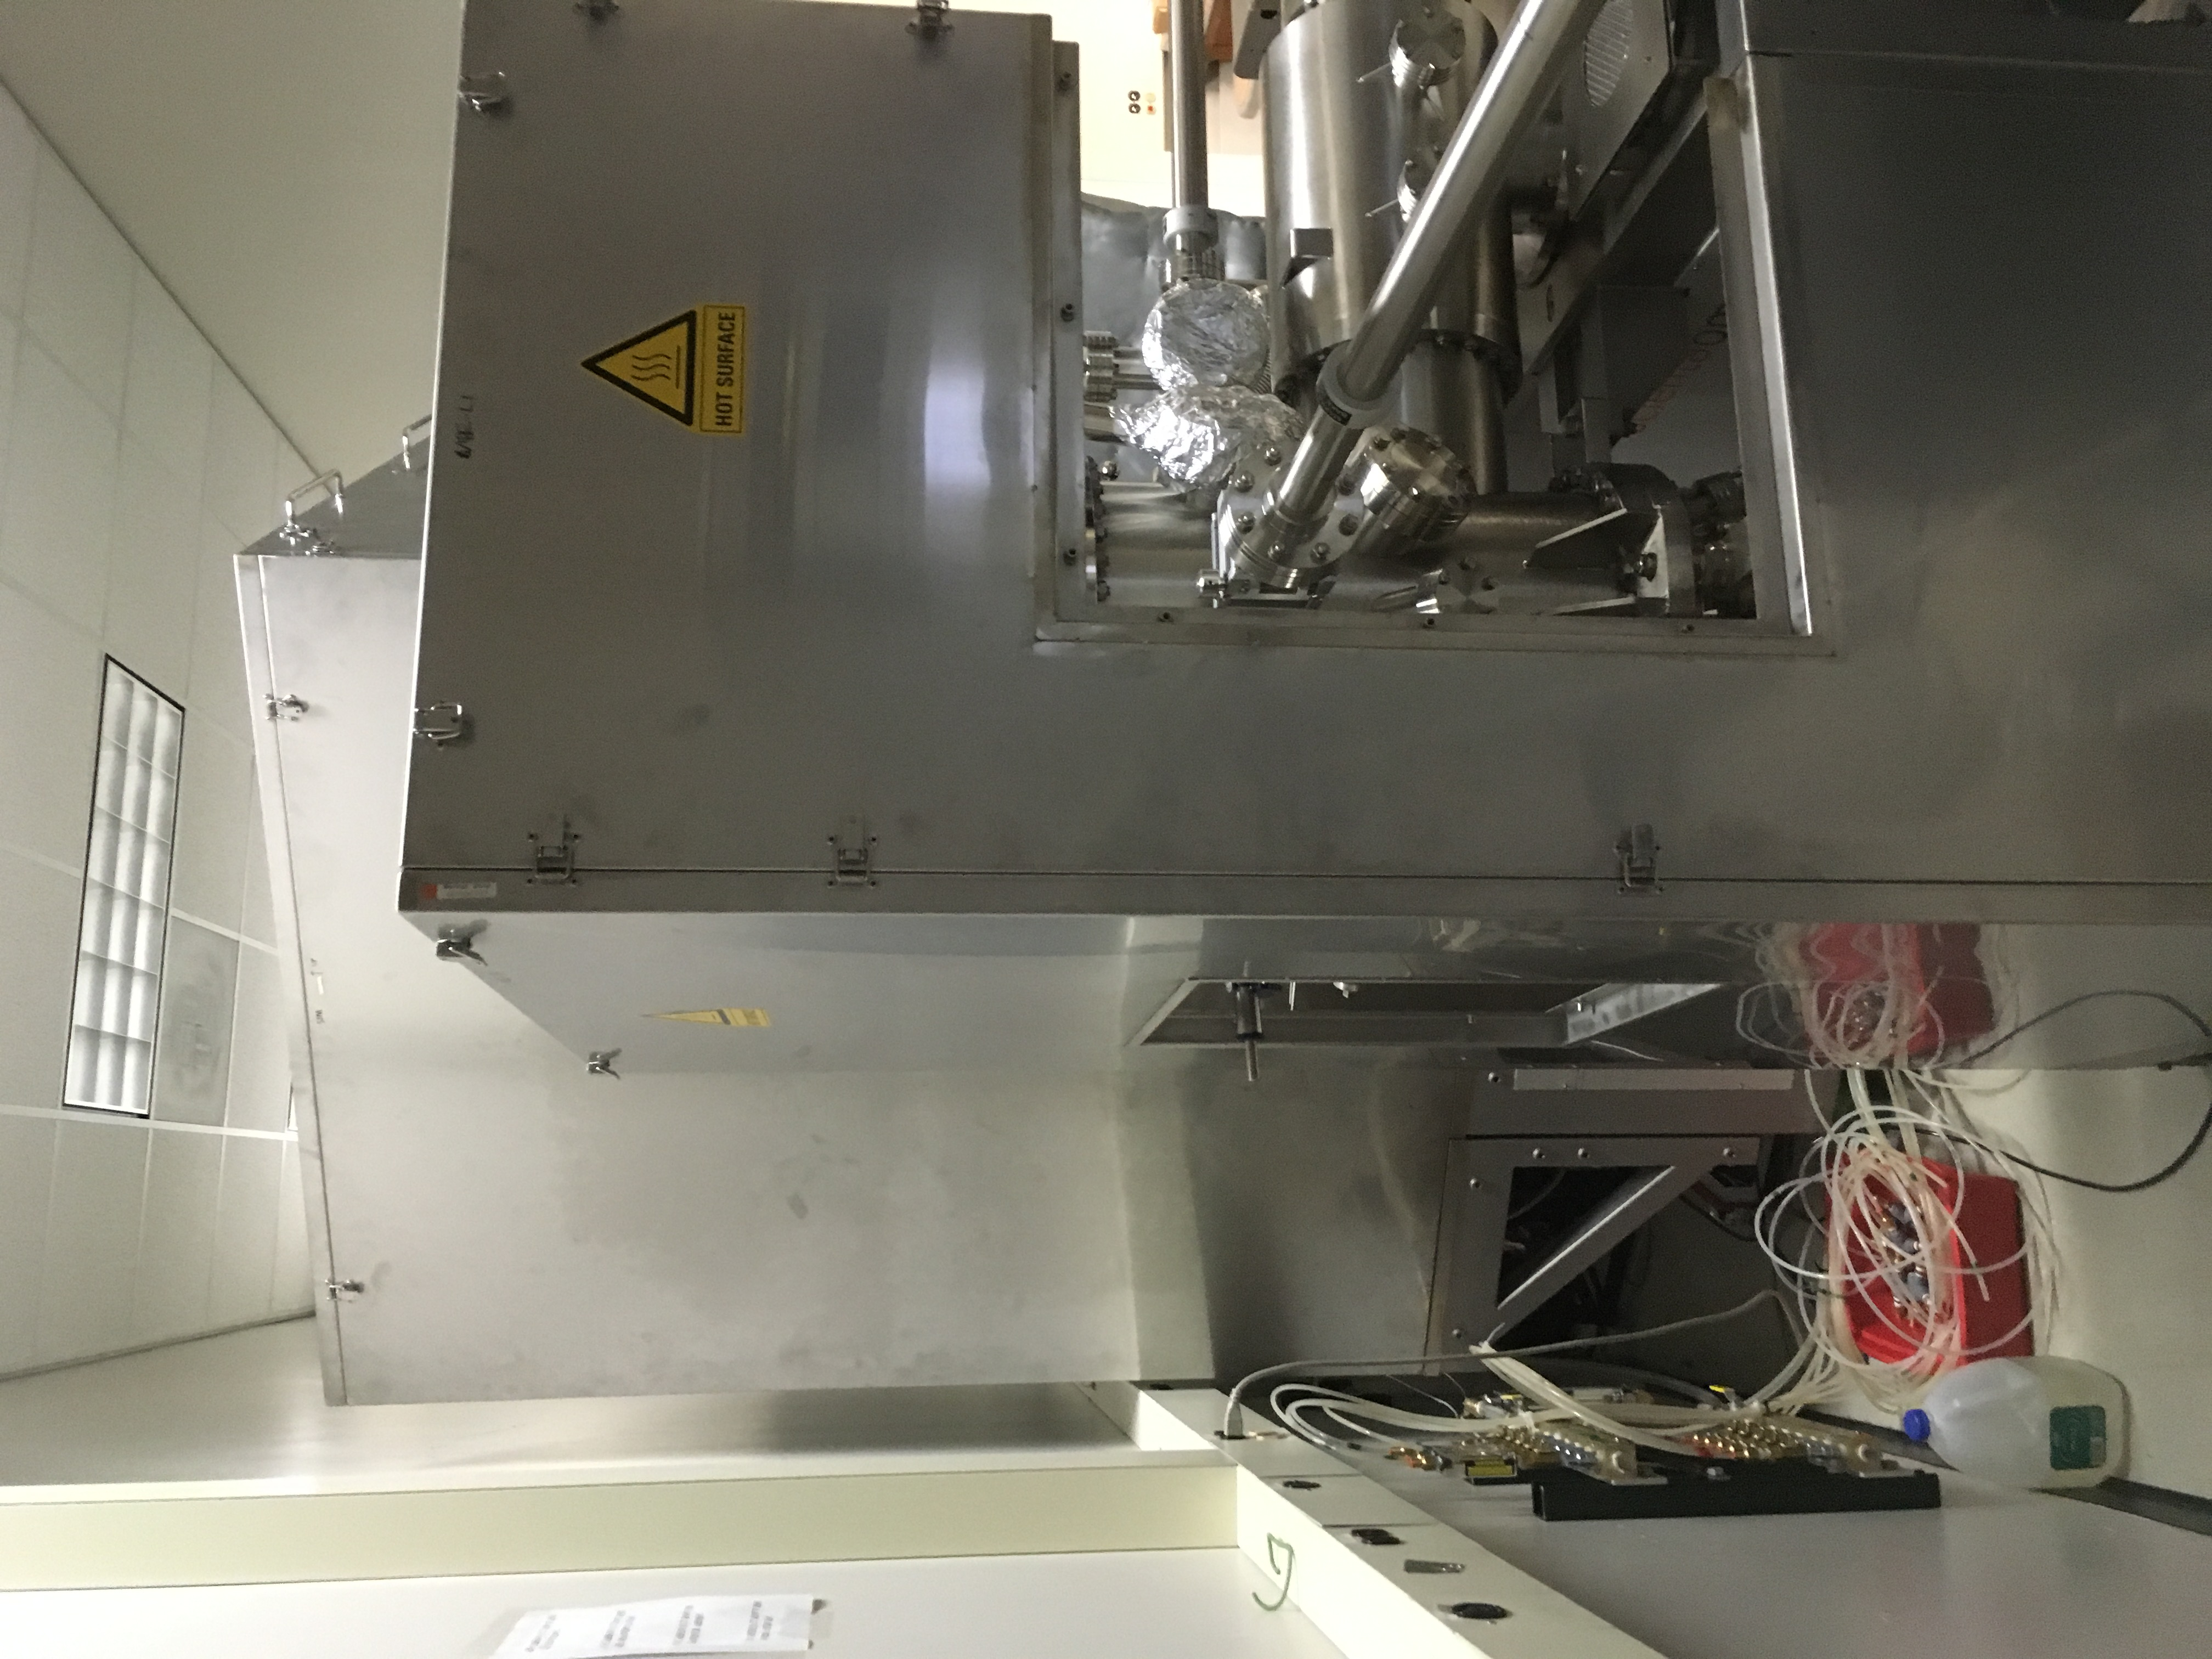
\includegraphics[width=1\textwidth, angle=270]{panels2.jpg}
	\end{minipage}\hfill
	\begin{minipage}[c]{0.33\linewidth}
		\centering
		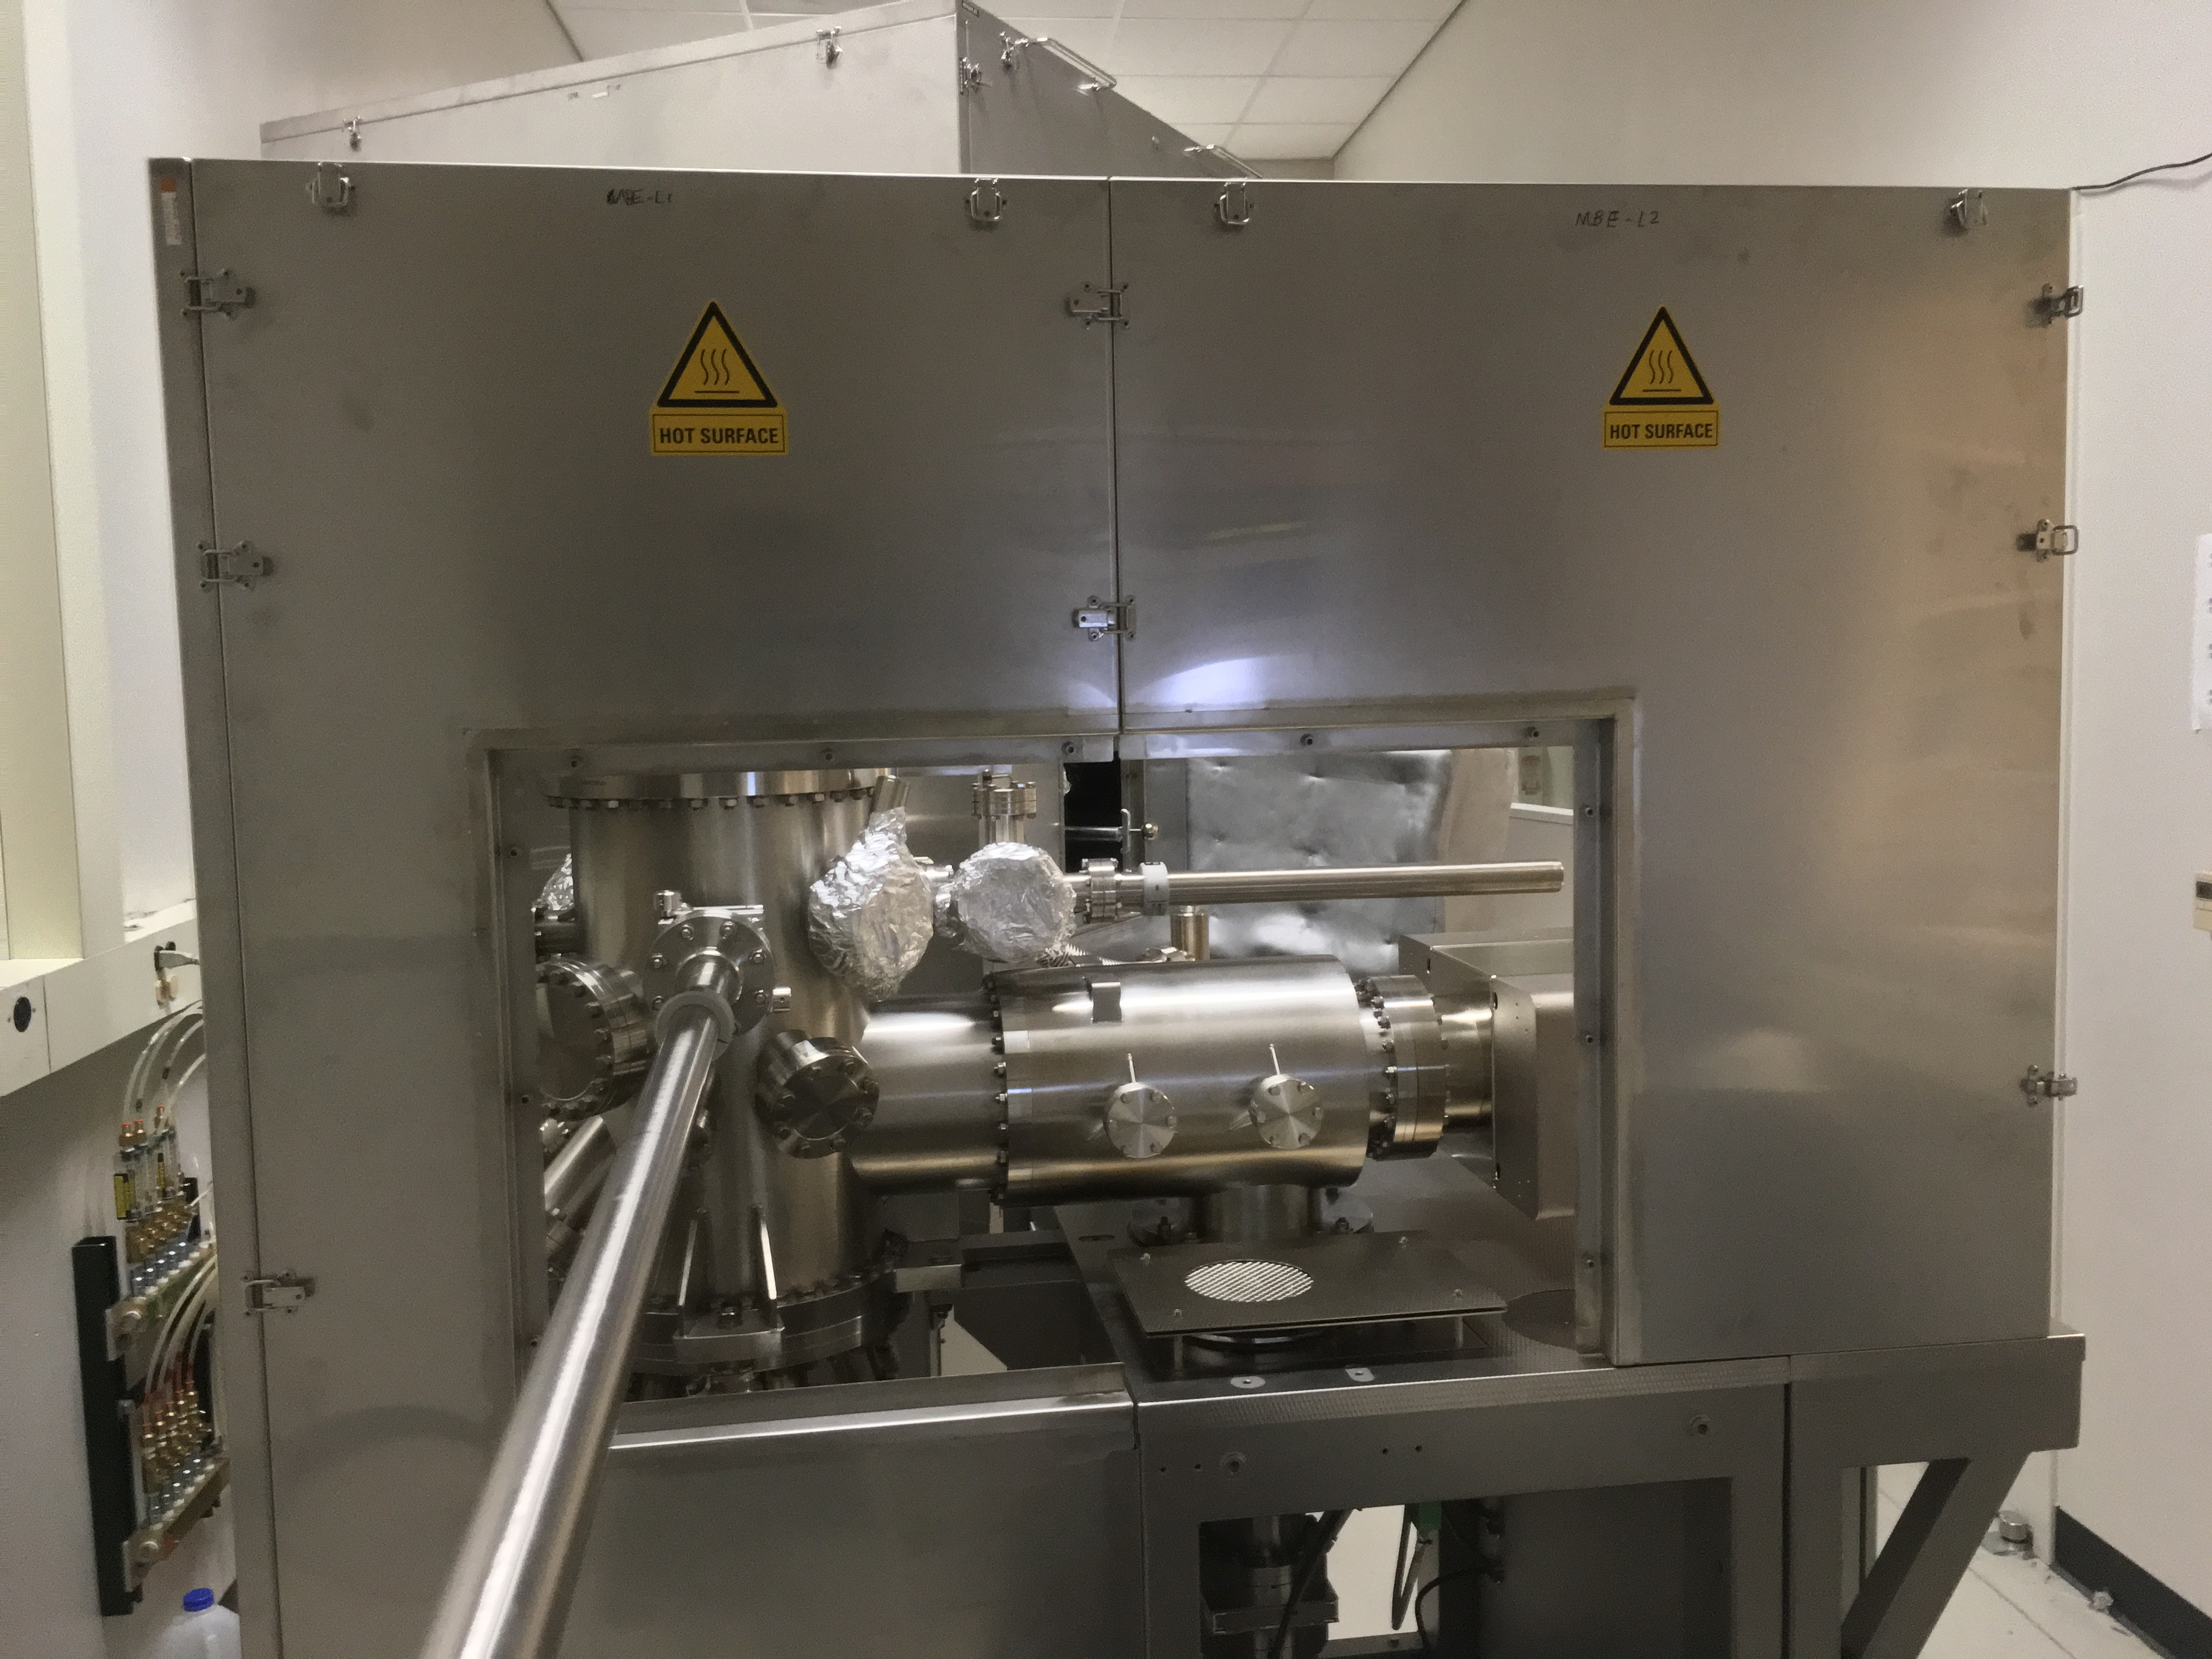
\includegraphics[width=1\textwidth]{panels3.jpg}
	\end{minipage}\hfill\vfill
	%-----------------------------------------------------------------------------
	\begin{minipage}[c]{0.33\linewidth}
		\centering
		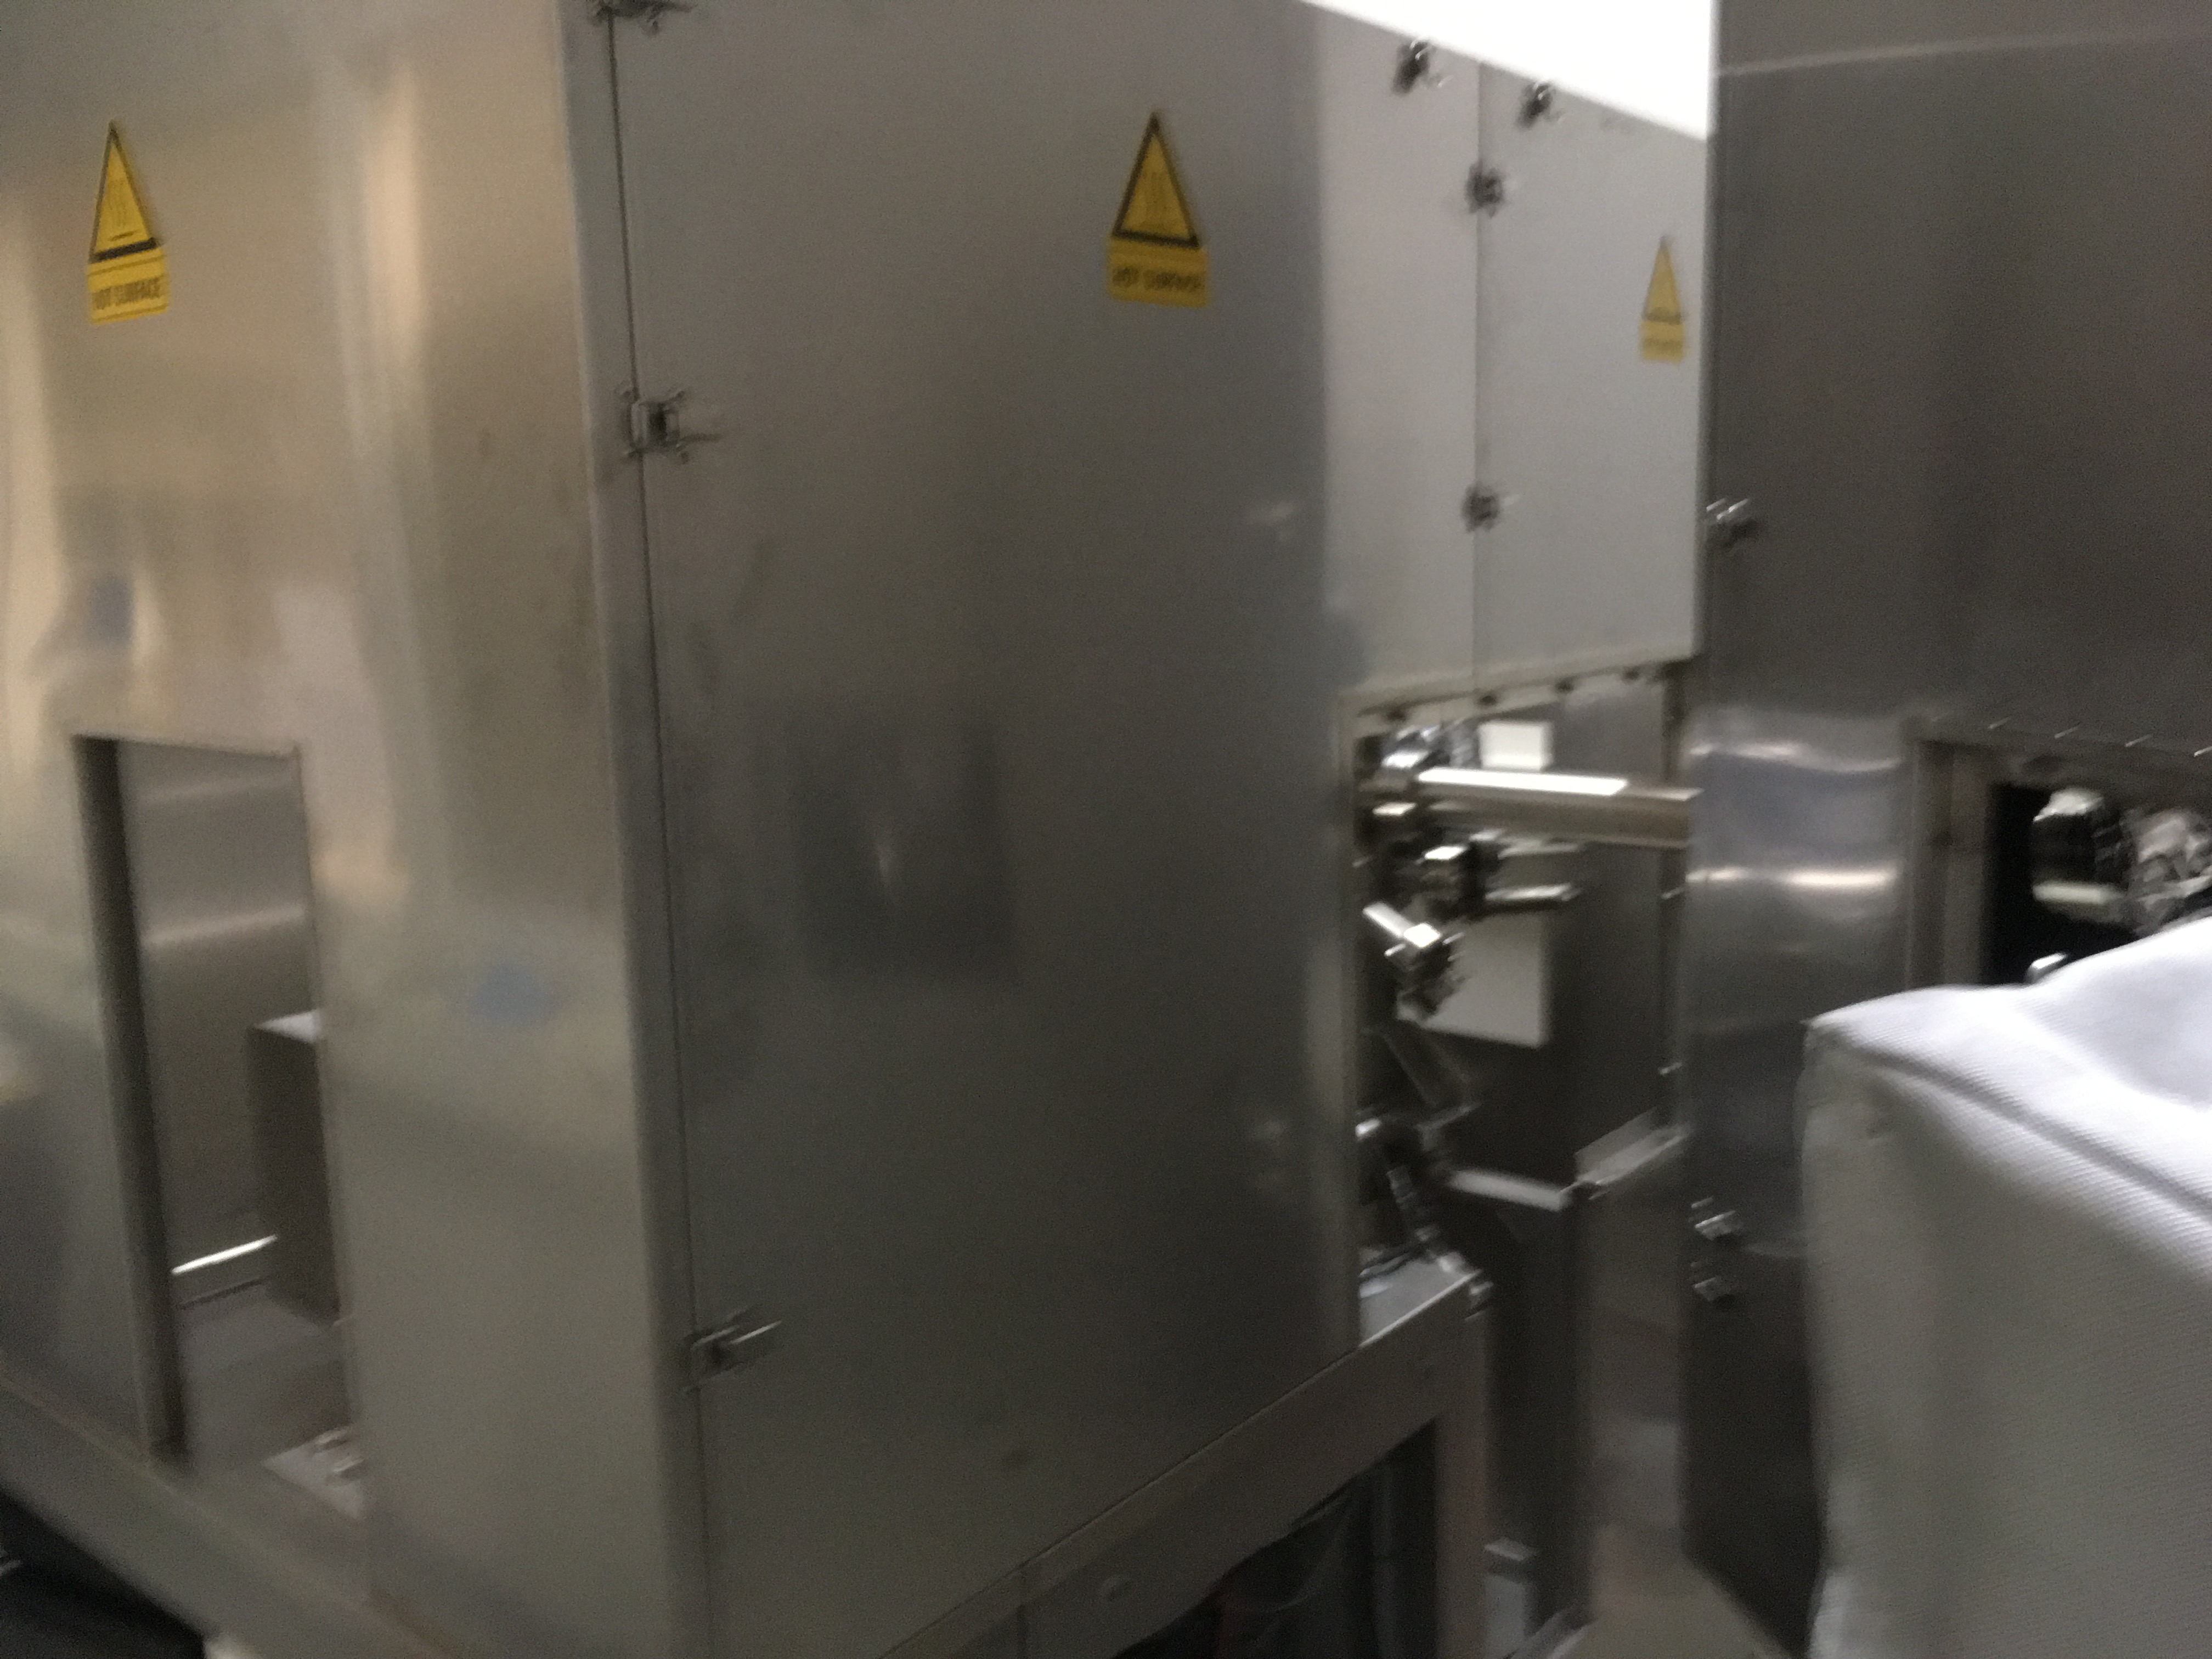
\includegraphics[width=1\textwidth]{panels4.jpg}
	\end{minipage}	\hfill %ADDING THIS FIXES THE ALIGNMENT!
	\begin{minipage}[c]{0.33\linewidth}
		\centering
		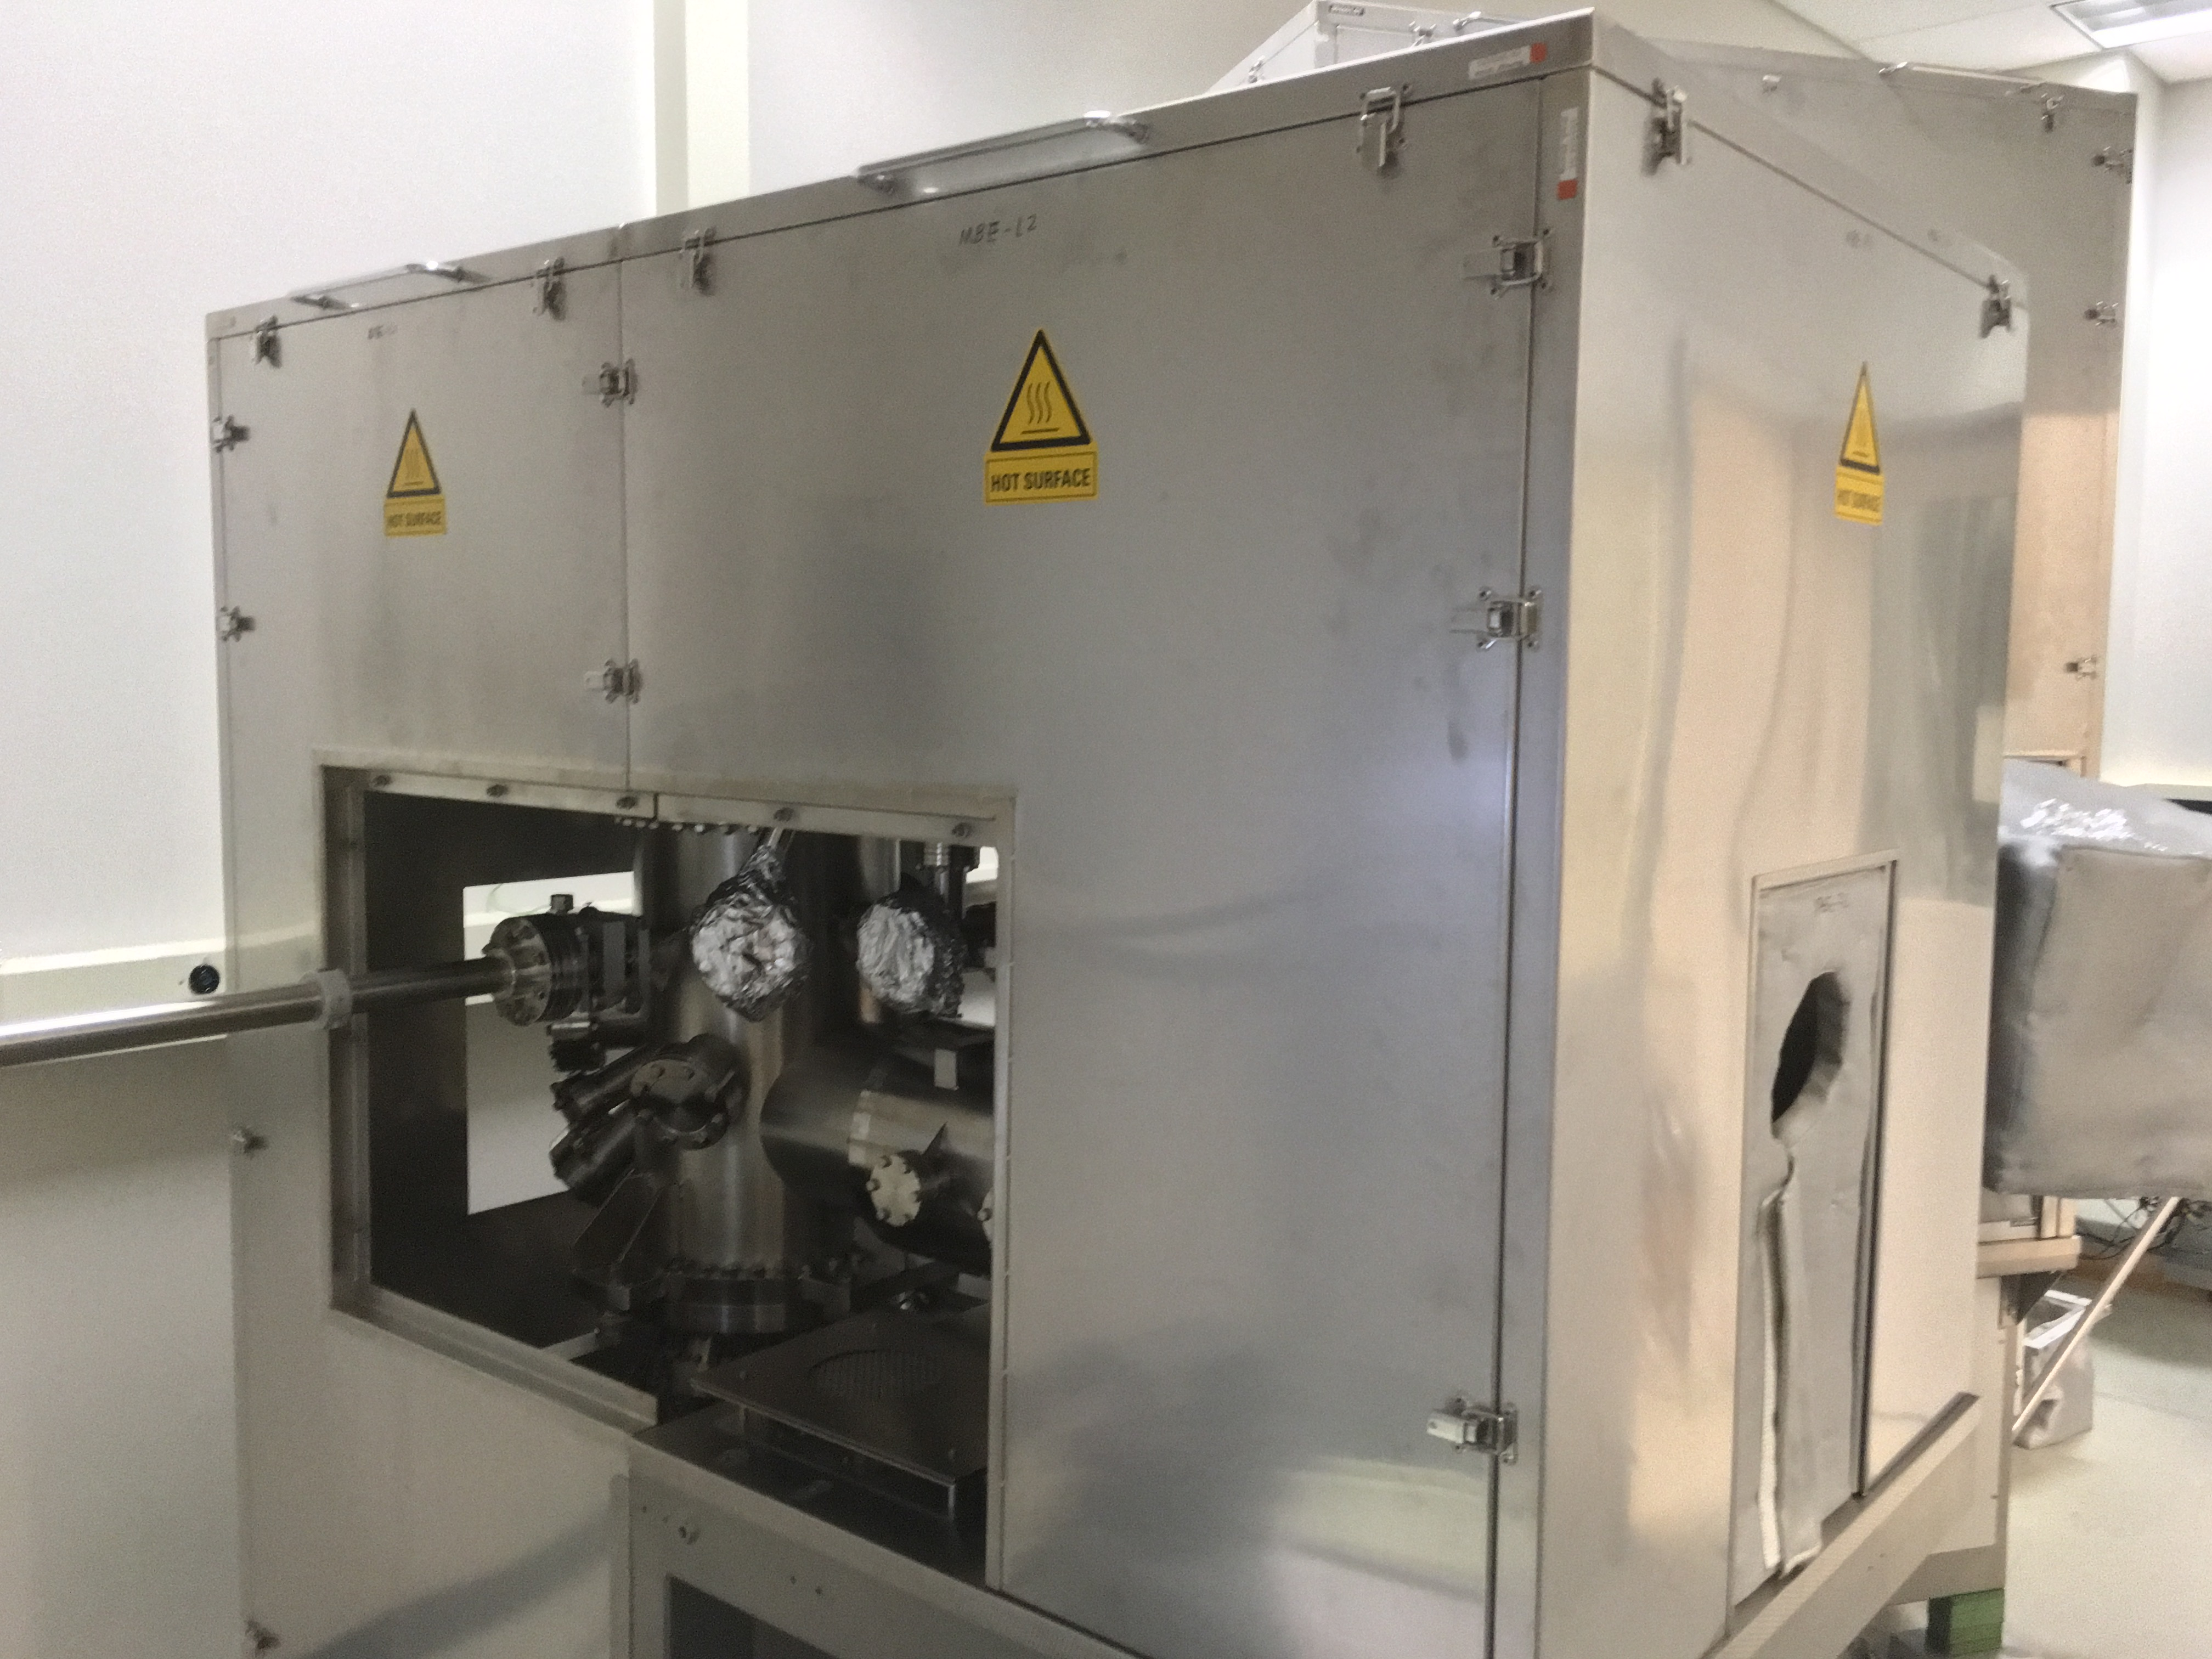
\includegraphics[width=1\textwidth]{panels5.jpg}
	\end{minipage}\hfill
	\begin{minipage}[c]{0.33\linewidth}
		\centering
		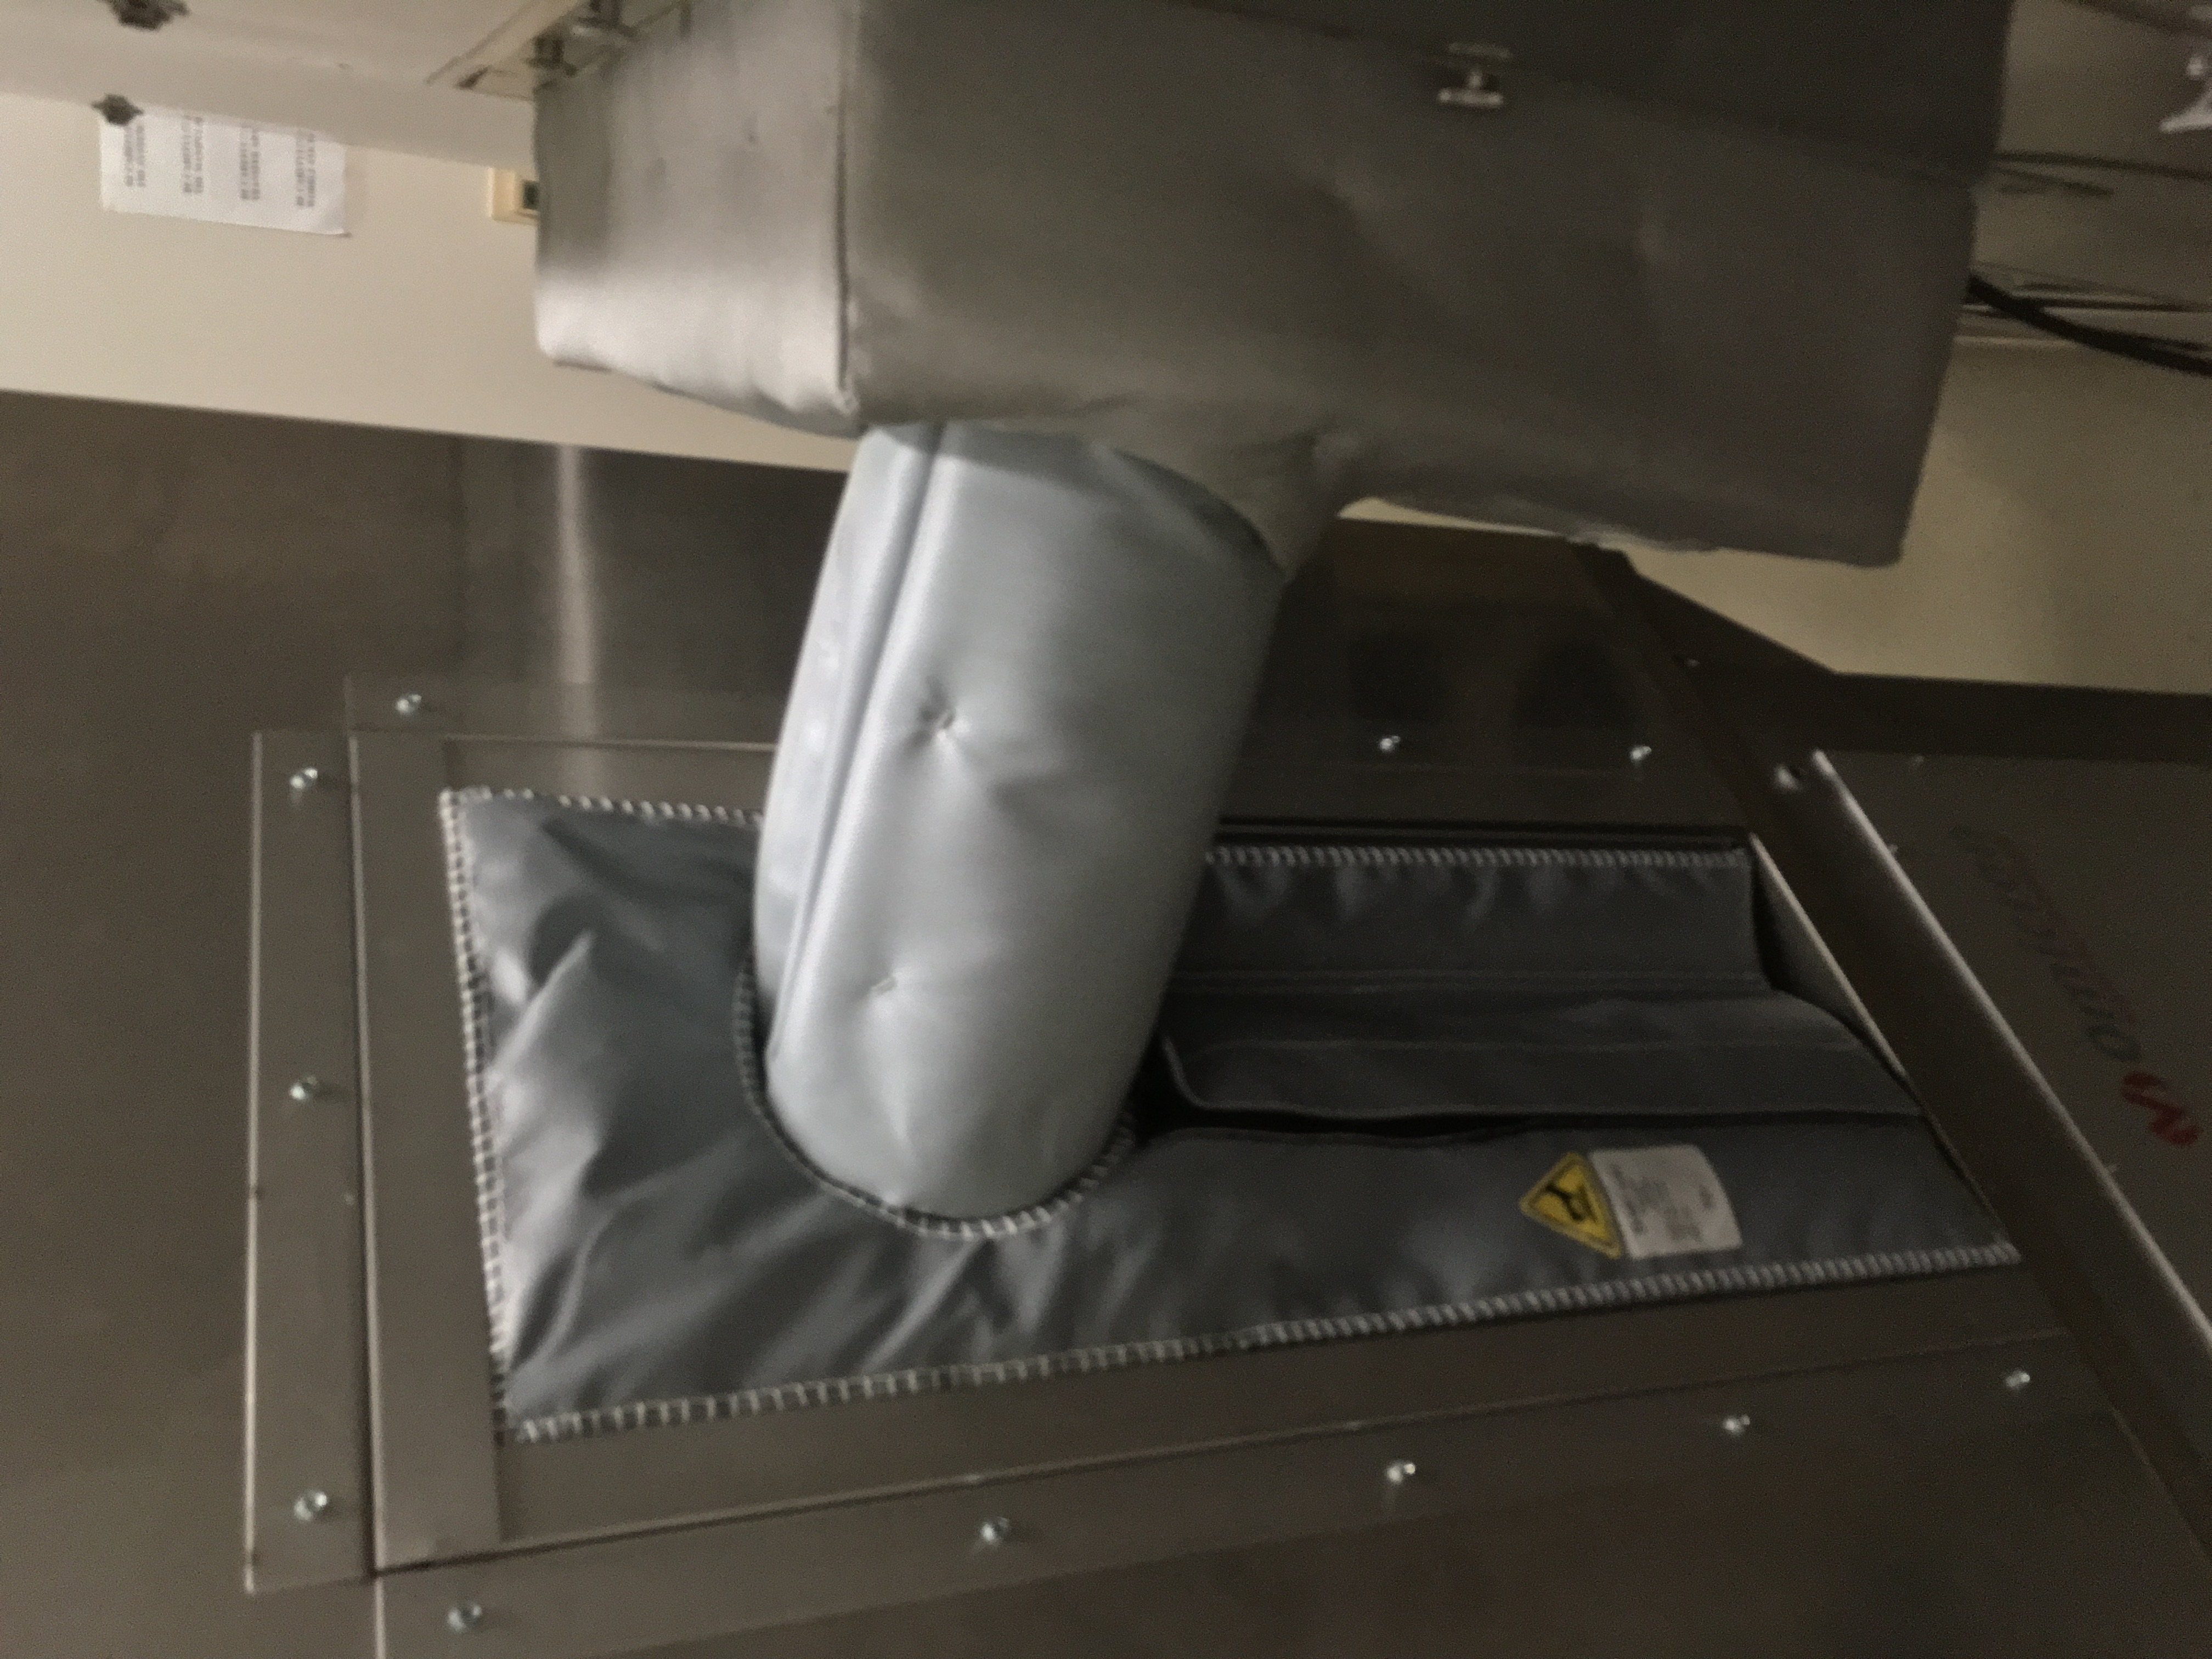
\includegraphics[width=1\textwidth, angle=270]{panels6.jpg}
	\end{minipage}\hfill\vfill
	\begin{minipage}[c]{0.33\linewidth}
		\centering
		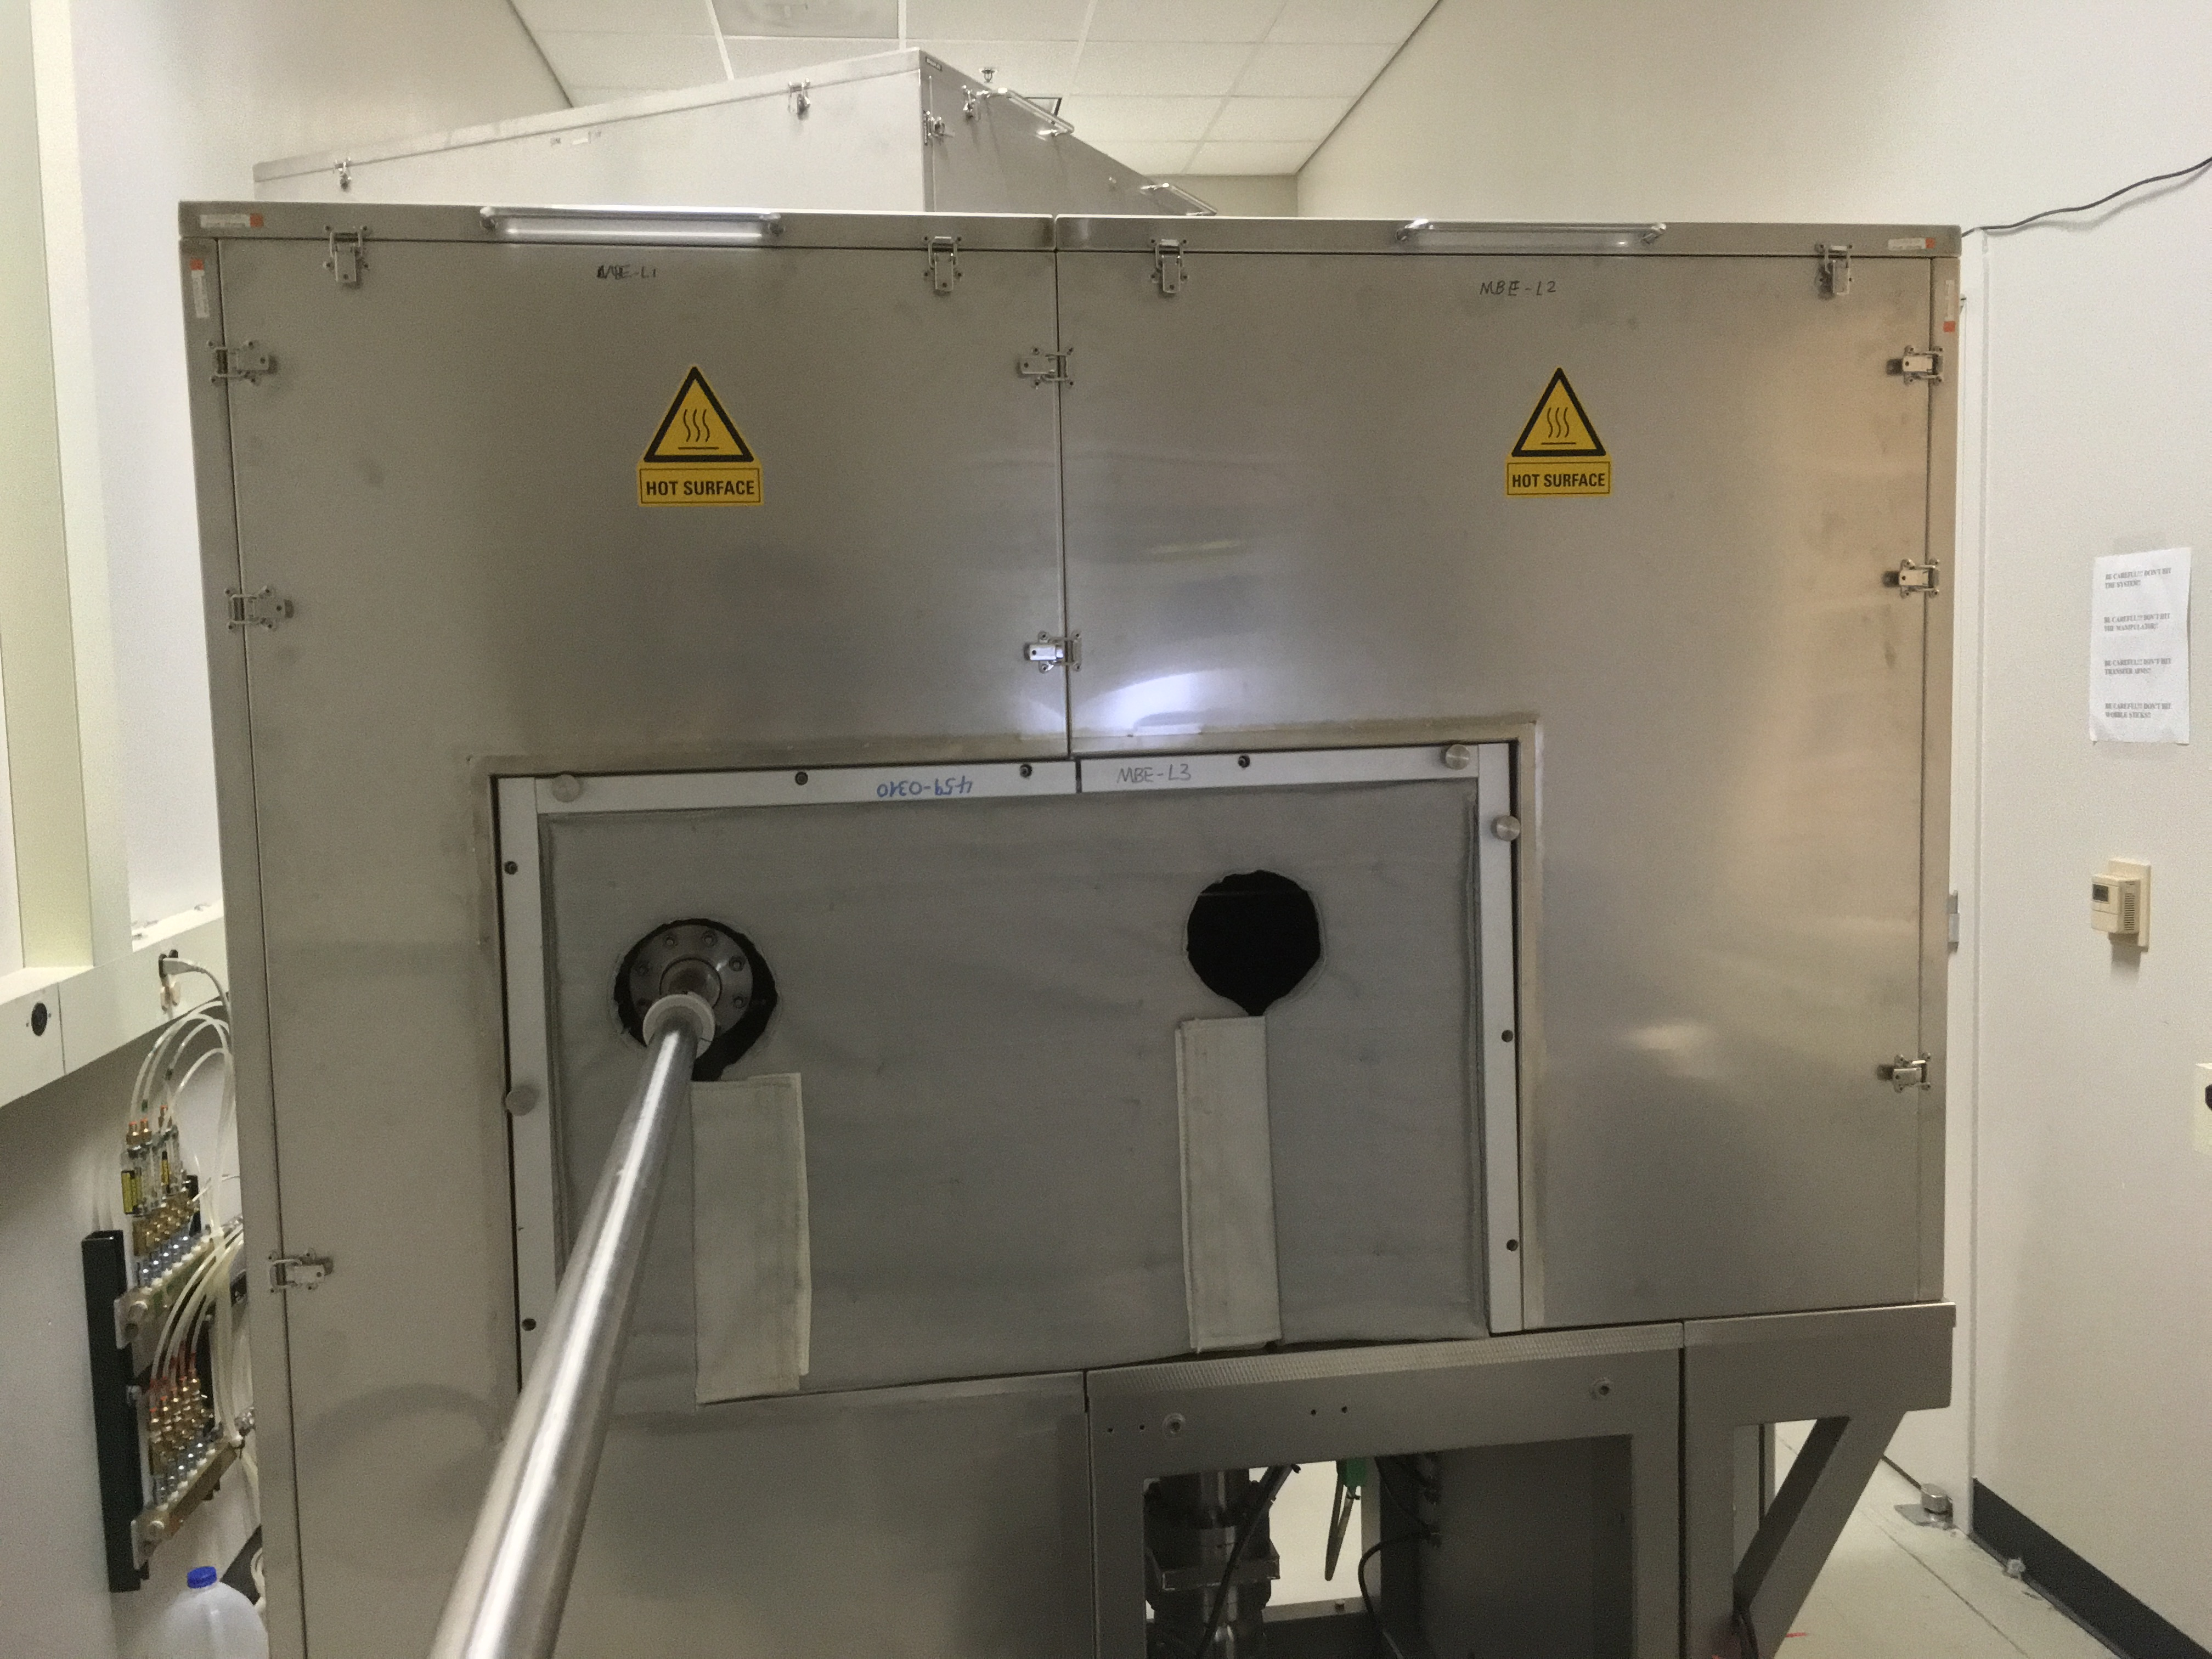
\includegraphics[width=1\textwidth]{panels7.jpg}
	\end{minipage}\hfill
	\begin{minipage}[c]{0.33\linewidth}
		\centering
		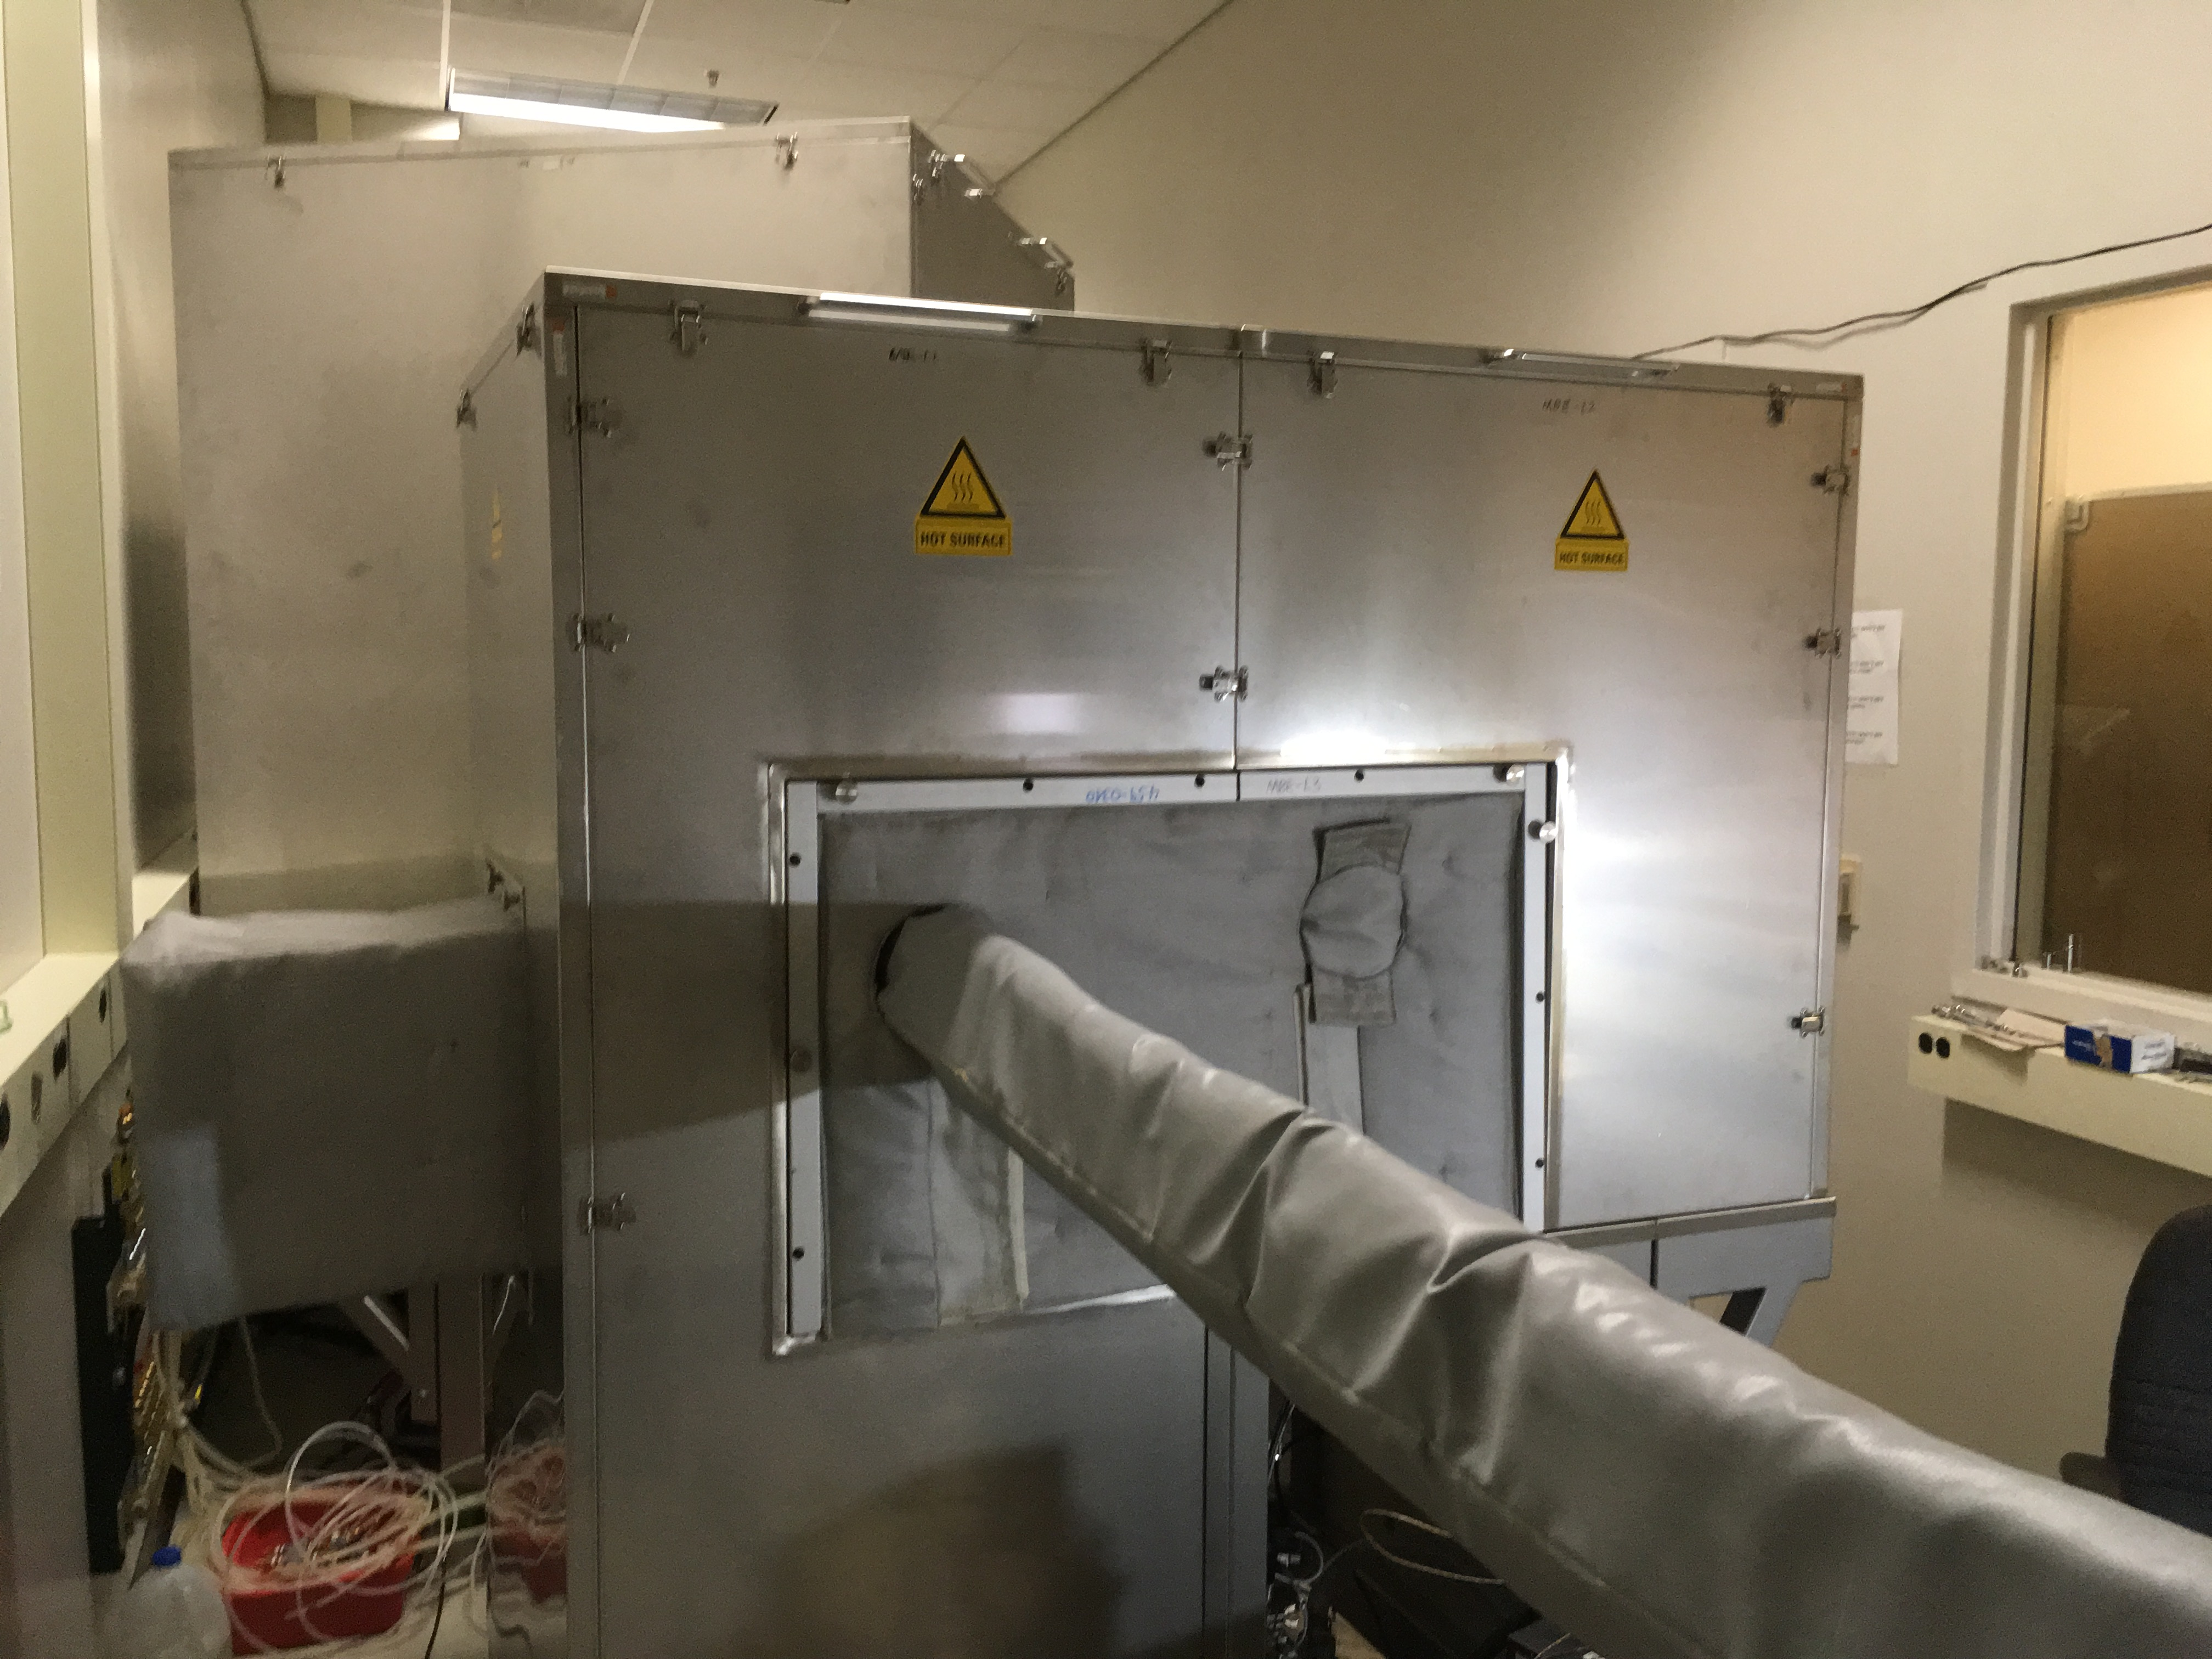
\includegraphics[width=1\textwidth]{panels8.jpg}
	\end{minipage}\hfill
	\begin{minipage}[c]{0.33\linewidth}
		\centering
		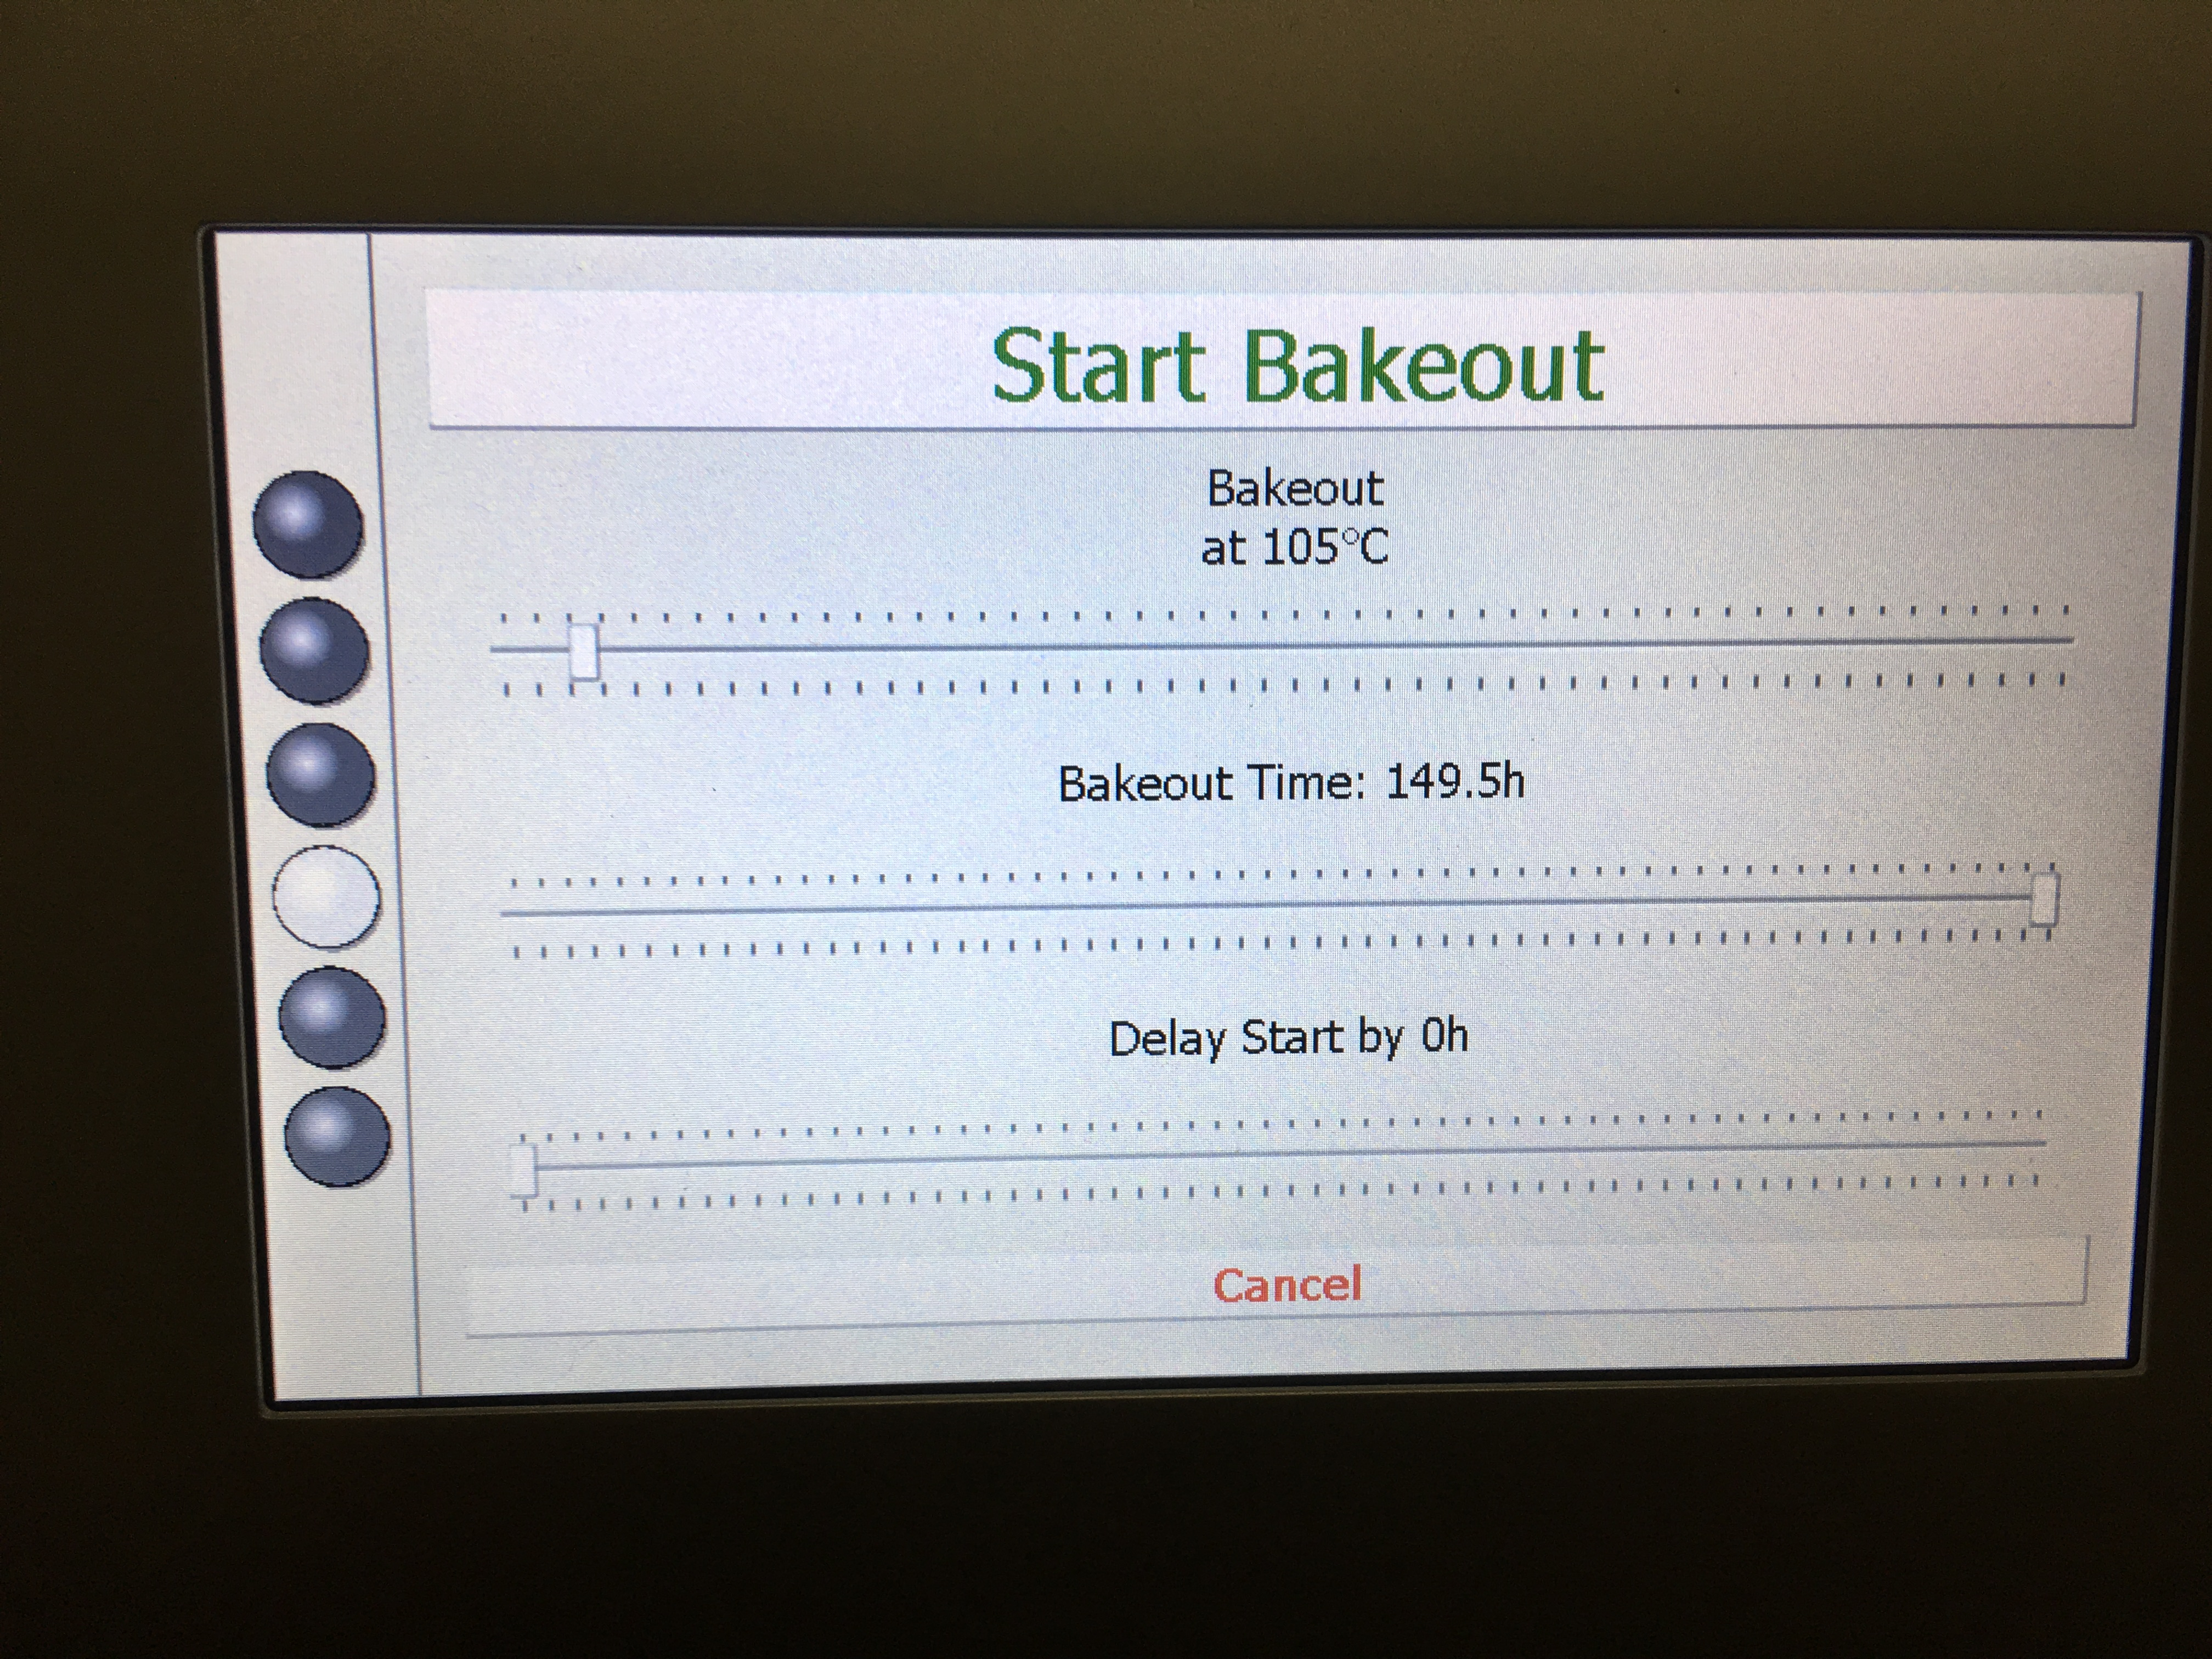
\includegraphics[width=1\textwidth]{panels9.jpg}
	\end{minipage}\hfill
	\caption{Order of panel assembly (read left to right).}
	\label{fig:gradual_heating}
\end{figure}




\item	Once system reaches good pressure (i.e. mid e-8mB), can start bakeout but first double-check the following things:
a.	Turbo pump is operating at full speed
b.	Ion pump and TSPs are off.
c.	Emission current on the ion gauge is set to automatic mode (see degassing ion gauge for details about using the controller).
\item	Start bakeout with set temperature of 105C. 
\item	Pressure in MBE chamber will start rising. Foreline pressure (the one in small display window) will stay constant (measured near the pump) at ~5.9e-1mB. It is expected to take about 90min for system to reach the 105C bakeout temperature. Should monitor pressure closely during this first period. Pressure will most-likely reach 2e-6mB. After see decreasing trend in pressure can monitor less frequently.
\item	As bakeout continues, dirt/impurities are being removed from the system and pressure will gradually drop. Monitor pressure periodically. Once pressure drops to ~8e-8 can probably stop bakeout. Bakeout will take about 72 hours.
\end{enumerate}

\section{Immediate Post-Bakeout Procedures}
Once bakeout is stopped:
\begin{enumerate}
\item	Degas ion pump:
a.	Turn on ion pump controller (at very bottom of stand) and press \emph{start HV} on controller touch screen. It will automatically select an HV at ~7kV. Will see pressure spike up to e-6 or e-5 range at which point immediately press \emph{stop HV}.  Then repeat turning on and off but each time should be able to leave ion pump on for longer intervals (pressure will be more stable). Eventually should be able to leave it on for 5-10min with stable pressure.
\item	Degas TSPs: 
Overide interlock (since degassing causes pressure rise and system will not allow to operate things otherwise). Then press “activate devices”. Once temperature cools to $<100$C, start degassing TSP filaments (3 of them).  
\begin{enumerate}
\item	TSPs are controlled by same touch screen controller as ion pump at bottom of stand. Select 1 of the TSP filaments (1,2, or 3) and hold “start TSP” until the display reads “firing”. It will automatically ramp up the current and then ramp it back down. Pressure will go up, might reach ~1e-6mB during the ramp. 
\item	Degas filaments 1 at a time at least 3 times. Use cycles of 1 ramp for each of 3 TSPs before doing a second ramp, instead of doing repeated ramps for only 1 individual TSP. 1 ramp cycle takes about 1min. 
\end{enumerate}
\item	Degas ion gauge: 
\begin{enumerate}
\item	Keep override interlock enabled and devices activated. Keep TSPs and ion pump off. This puts a higher current through the 2 filaments of ion gauge to help clean it. On ion gauge controller at top of stand, press book icon until reach \emph{ion gauge menu} $\rightarrow$ press checkmark to select this. Press book icon until reach \emph{filament} and see which filament is selected $\rightarrow$ press \emph{x} to go back to menu. Press book icon until reach \emph{emission} $\rightarrow$ use arrows to find \emph{medium degas} $\rightarrow$ press checkmark to select. Repeat for the other filament (there are 2 filaments since 1 is a backup, only 1 filament is used to read the pressure at a time).
\item	To repeat for other filament, need to turn switch pressure reading to that filament: Press checkmark and x at same time to turn ion gauge off. Then press book icon $\rightarrow$ \emph{ion gauge menu} $\rightarrow$ checkmark to select. Book icon $\rightarrow$ \emph{filament} $\rightarrow$ arrow to chose other filament $\rightarrow$ checkmark to select $\rightarrow$ \emph{x} to go back to main menu. Book icon $\rightarrow$  \emph{emission} (this allows to choose emission current used $\rightarrow$ checkmark to select \emph{auto}. Wait until see a pressure reading show up again, now the other filament is on. Now proceed as before to verify that desired filament is on and degas it. One filament degassing takes 10min. 
\item	Change the settings to use the filament that used before did degassing: book icon $\rightarrow$ \emph{filament} $\rightarrow$ arrow to chose filament $\rightarrow$ checkmark $\rightarrow$ \emph{x} to go back to main menu.
\end{enumerate}
\item	Now since have degassed the major things, can turn on ion pump. If turn on a bit later is also ok.
\item	Once system temperature reaches ~80C, remove the small round covers to speed cooling.
\item	While ion pump is still off, run TSP filaments one by one for 1 ramp every 30min. 1 ramp takes just 1 min and will auto shut off. Will still have some degassing occur and pressure could rise to low e-7 range. Running TSPs will help improve the vacuum. After finish running TSPs, remember is disable the interlock override so that the safety feature is enabled.
\item	Once temp. reaches ~70C, open flaps on flexible bakeout panels and heated tubes but do not remove them.
\item.	At 60C, remove all flexible bakeout panels and tubes.
\item	At 50C, remove all metal bakeout panels.  Remember to finish running all 3 TSPs for 1 ramp cycle. By this time, pressure should have reached low e-9 range.
\item	Wait until most system components are only slightly warm to the touch before doing any other work on the system. While waiting, can connect the electronic cables for the evaporators and the LEDs for the viewports.
\item	Once pressure reaches low e-9mB range, will need to perform more degassing. All of these are not possible to do the same day as finishing bakeout. Generally allow about a week to finish all the degassing.
\textbf{Before any degassing, make sure that there is a blank on the heater stage!}. To transfer a blank to stage, need to first put back the black magnetic coupler onto the transfer arm as follows:
\begin{enumerate}
	\item Close [FEL,MBE] valve (so when reinstall coupler don’t accidentally push transfer arm into MBE). 
	\item Open [FEL,turbo] metal valve to let turbo pump on FEL.
    \item Slowly put the black coupler onto short transfer arm. After on at some distance, arm will begin to move. Move in slowly until feel the resistance of forks touching the valve. Gently push on coupler to try to install coupler a little bit further in. Sometimes coupler will couple before it is far enough on the transfer arm. In this case, do not apply too much force, pushing arm against valve. To fix this, when move the blank into MBE heater stage, can apply some force when arm is locked to heater stage to push coupler in further. There is less damage risk, pushing against heater stage (since it’s made for that) than pushing against valve.
	\item 	Close [FEL,turbo] metal valve and close [FEL,MBE] valve.
    \item While waiting for system to cool, reconnect the evaporator electronic connections.
	\item Once ion pump is relatively cool, close main gate valve (touchscreen) so system is running only on ion pump. Leave turbo running since will need it for degassing.
	\item Need to wait for system to cool (can judge by heater stage temperature, readout on touchscreen or touching various system components) before transfer blank to heater stage.
\end{enumerate}

\item	Degas evaporators (see procedure). 
\item	Degas heater stage (see procedure). \textbf{Make sure the evaporators have been degassed first, otherwise they will contaminate the heater stage!}
\item	Run TSPs, 1 filament at a time, to help reduce pressure which will have increased due to degassing.  To run: override the interlock and press \emph{activate devices} on the interlock screen on touch screen. Then on very bottom touch screen, select which TSP filament want to run, hold “start” until displays “firing”. TSP will automatically run and shut off. When run TSPs, the pressure will increase fast and then decrease. This pressure is due to the titanium being sublimated which then absorbs other particles and sticks to the chamber walls.
\item	When pressure reaches 1-2e-9mB, turn on ion pump (press \emph{start HV}). If pressure spikes up too high, immediately turn off ion pump. 
\item	If were able to turn on ion pump successfully, close gate valve on touchscreen (this is valve btw. MBE chamber and turbo pump). Now the system will be pumped only by ion pump.
\item	Vent turbo pump (make sure gate valve is closed!) and turn off turbo to let it rest.
\item	With the ion pump running, should be able to reach e-10mB pressures (without L N2 filling).
\end{enumerate}

\section{Degassing Se Evaporator}
First, the power supplies need to be reconnected:
\begin{enumerate}
\item Need to have 3 boxes: the large grey Eurotherm box and 2 small boxes (which work together as 1 power supply + temperature controller is a separate box). Connect the EC (small box) connections to the Se evaporator protrusion that is labeled EC. Make sure the 2 terminals (metal loops) do not touch when are fixed in place! Need to tighten gently but at the same time make sure that the terminals do not move.
\item Connect the connections from Eurotherm box to the other protrusion on evaporator. When connecting the terminals polarity doesn’t matter. Be very gentle when tightening the screws. The connections are very delicate and bend very easily! Connecting the power supplies is inconvenient due to the small space available near the Se evaporator.
\item For power cords: connect the 2 small boxes (power supply and temperature controller) to the surge protector and connect surge protector to a socket on the short wall of the room. Connect the large Eurotherm power supply using the orange extension cord directly to a socket on the long wall of the room (under the large Cutler-Hammer power breaker). This is so that are using different circuits and don’t overload anything.
\end{enumerate}
Now can begin the degassing:
\begin{enumerate}

\item On EC controller (small boxes) on the Solo temperature controller, at first set the voltage set dial to 1 (read in the small window of dial, the main knob should line up at 0). Setting to 1, makes the maximum voltage = 3V (or $10\%$ of 30V). Then when reach higher temperatures, if see that actual temperature doesn’t follow fast enough, increase the voltage set dial gradually. Once reach close to 60C, have the voltage set at 2. If initially set the max voltage too high, then temperature might overshoot in an uncontrolled way.\\\\
For bottom large (Eurotherm) controller, hear the “heating power output limitation” is equivalent to the voltage set on small controller. At first, set this to align with the sharpie mark. Later will need to increase it gradually to be able to heat to higher temperatures.
\item Gradually increase temperature on both controllers in 5-10C increments. If there is significant degassing at lower temperatures, then wait a while before further increasing temperature. It is better to degas as much as possible at lower temperatures at which the Se will not be evaporating than try to do all degassing at high temperatures where are also consuming the Se. On the Eurotherm controller, will need to adjust the heating power knob (increase it past the sharpie mark) for there to be enough power to maintain the desired temperature. Otherwise the temperature actually begins to decrease! But do not put too much heating power because that will result in temperature to rise too fast and overshoot.
\item In 2016 bakeouts, we degassed in the range 50-60C for top controller and 110-145C for bottom controller. Increased top by i.e. 2C increments and bottom by 5C increments. Want stay in this temperature range for less than 1 hour, otherwise will be consuming too much Se source. Therefore, do not wait too long between incremental increases.  Stay at the max setting: 60C and 145C for about 10min, then gradually tune it down. 
\textbf{Note: Degassing procedure probably needs to change if plan on using much higher cracker temperatures}.\\\\
During degassing pressure may rise significantly since Se is easy to evaporate. Pressure may rise to e-8mB range. If pressure rises to high e-8mB, need to be very careful and perhaps tune down the temperature.
(When degassed on 10/13/16, pressure stayed in the e-9mB range even at the max temperature settings of 60C and 145C).
\end{enumerate}
\section{Degassing E-beam Evaporators}
The E-beam evaporators will be degassed twice. The first time, no water cooling and no HV is used. This is to degas the filaments. During the second degas, we use both the water cooling and HV and degas the evaporation source. For the second degas the procedure for W and Sn evaporators are different.
\subsection{Degassing E-beam evaporators without water cooling and HV}
The initial degas procedure is the same for both  evaporators. \textbf{During this we keep HV off!} This is extremely important, since we have the water cooling off. Otherwise we will overheat the evaporators.
\begin{enumerate}
\item	Turn off ion pump to avoid potential damage due to high pressures from degassing. 
\item	Make sure evaporator shutters are closed, otherwise too much heat is introduced into the MBE chamber.
\item	Make sure that have properly connected the electronic cables to the evaporators: red goes to HV (the rod), black to flux monitor terminal, 4-pin connector to 4-pin port, grounding cable should be put under the nut on the flux monitor port protrusion and nut gently tightened with wrench.
\item	Will degas without water cooling so evaporators can reach a high temperature enabling to remove contaminants. This means must make sure that HV is kept off! Otherwise an electron beam will heat crucible/rod and thus evaporator to unsafe temperatures (the temperature reading on evaporator controller does not accurately portray temperature near crucible or rod when that is heated by and electron beam).
\item	It is most time efficient to degas both evaporators at the same time. Gradually increase FIL current on both evaporators to 1.6A. 
\item	Wait for evaporator temperatures to rise which will cause pressure to rise. 
When did degassing on 10/5/16 on W evaporator, at first there was significant flux which later went to <0nA. This was probably the filament degassing, since we did not degas filament on this evaporator after changing it. The reason that we see no flux when degas the entire evaporator is that the filament locally reaches much higher temperatures than the evaporator body. These high temperatures of filament are enough to cause the dirt on filament (if haven’t degassed it previously) to ionize and register a reading on the flux monitor. The evaporator body reaches just 200-300C which is not enough temperature to ionize the dirt coming from it.
\item	During degassing, keep pressure below 9e-7mB. If pressure rises above this, decrease FIL to 1.5A or 1.4A. If temperature is rising too slow, can increase FIL in 0.1A increments. Note that there is a delay between increasing FIL and temperature increase. Once temperature reaches 220-240C and pressure stabilizes and starts decreasing, degassing is complete. (Manufacturer suggests to tune FIL to 2A and just wait 1-2hrs for temperature to rise to 200-300C, but we find this causes too fast temperature rise which causes too high of pressure so we use lower FIL currents). Unlike the STM thermal evaporators, here only 1 ramp up cycle is necessary to degas.
\item	Gradually tune down FIL to zero. Evaporators will take a while (several hours to cool).
\end{enumerate}


\subsection{Degassing W Evaporator with water cooling and HV}
\textbf{Note: This only applies to the W evaporator. Does not apply to Sn because that one uses a crucible!}.\\\\
\textbf{This is done after bakeout and degassing both e-beam evaporators w/o water cooling (and w/o HV) and the resistive heater stage.}
\begin{enumerate}
\item	Turn on turbo pump the day before plan to do this degassing. Keep ion pump on for now.
\item	Make sure water cooling is running properly.
\item	Make sure turbo pump has been running. Open gate valve: this will result in a pressure spike (i.e. into low e-9mB range) which is normal. The pressure should fall back down to e-10mB range after fill the cryostat. 
\item	Turn off ion pump to protect it from high pressures/contaminants due to degassing.
\item	Fill L N2 cryostat which acts as a pump to help maintain low pressures during degassing. It also keeps the chamber walls cool. This is important since there is concern that using evaporators w/HV on radiates a lot of heat which would heat up the chamber walls and could damage the coating on the walls. The company suggests to always use L N2 when using evaporators with HV on.
\item	Gradually tune HV to 2000V. Slowly increase FIL until get a stable FLUX of 10-20nA. This will occur after the dirt from the rod has been degassed and is slight evaporation of rod occurring. 
On 10/12/16, reached 10nA FLUX at FIL = 1.88A, EMIS=26.6mA. Reached 17nA FLUX at FIL=1.90A, EMIS = 28.0mA and held at this setting for 15min. Pressure stayed in high e-10mB or 1e-9mB range throughout the degassing.
\item	Run at this setting which has stable FLUX of 10-20nA for 15min. Do not run longer because are evaporating and consuming the rod here. While running, refill cryostat if necessary (if no vapor coming out of outlet, then need to fill).
\item	Tune down FIL and HV.
\end{enumerate}

\section{Degassing heater stage}
\begin{enumerate}
\item	If evaporators have not yet been degassed, do that first. We degas evaporators before heater stage since there is no cover that can protect stage from dirt so it gets contaminants on it while degassing the evaporators.
\item	Make sure there is a blank installed on MBE heater stage. 
\item	Make sure MBE pressure is in low e-9mB range before attempt to degas heater stage. If pressure is in mid e-9mB range, could still try degassing but pressure will most-likely rise into unsafe levels ($>5e-7$mB) before are able to reach 915C. It might make the second degas attempt easier though. Do NOT fill cryostat, it must remain at room temperature. Pressure will likely not be low enough if the evaporators have just been degassed. Need to wait until evaporators cool before try degassing heater stage. 
\item	Make sure evaporator shutters are closed, to protect evaporators from dirt coming off the heater stage which is above them.
\item	Make sure ion pump is off to protect it from any high pressures and dirt coming from the degassing. To turn off press \emph{stop HV} on ion pump controller.
\item	Make sure viewport metal shutter is closed to protect viewport from the high temperatures.
\item	On touchscreen go to “bias selector” screen and choose “resistive heating”. Then turn on heater control box, press preview, make sure see 28.7 voltage value (+/-0.2) and 0.02(or close) current value. If values are different, then do not proceed further. Press \emph{out} on heater controller: this turns on the output to the heater stage. Push \emph{fine} to be able to have better control when turn the dials. 
\item	Tune the current up in 0.5A steps (or lower increments if pressure increases too much).  Voltage will increase automatically. Heater stage temperature is displayed on the touch screen. Temperature will increase as increase current. Keep pressure below 5e-7mB, but preferably in mid-e-8mB while current is below 8A.
\item	At first as increase current in 0.5A steps, should observe increases in pressure, followed by decreasing back down to the value before did the increase. Once heat sample stage to ~600C, pressure will most likely gradually creep up without decreasing. When see pressure gradually creep up, just keep increasing the current after waiting for a few minutes. The continuous pressure increase is because higher temperatures, stage is also significantly heating the MBE chamber walls and they will start degassing also. Since there is a large amount of walls, pumps will not be able to overcome this degassing. This is why it is important to start the heater stage degassing at a low base pressure.
\item	Continue tuning up current (while keeping pressure below 5e-7mB), until heater stage reaches 915C. The current needed will most-likely be 10.66A. Do not allow heater stage to heat above 917C (1190K) since the absolute upper limit that the heater stage can withstand. 
\item	Degas at 915-917C for 3-5 minutes. Note that the temperature tends to slowly increase even after have already set the current to 10.66A so monitor the temperature closely. If at any point it becomes $>917$C, decrease the current immediately. Pressure is unlikely to decrease and may even creep up. This however does not mean that degassing is ineffective. Pressure is high because the heating of heater stage to such high temperature heats the MBE chamber walls which start degassing a lot also.
\item	Gradually tune down current to 0. Can tune down faster than tune up, but still do it at a controlled speed so pressure and temperature doesn’t fall too fast. Can turn off “fine” to tune down, but in that case, turn knob very slowly.
\item	To shut-off: on heater controller, deactivate \emph{out} button, deselect \emph{fine}, turn off controller box. On touch screen \emph{bias selector} screen, select \emph{grounding}.
\end{enumerate}
Some other notes:\\
At 200C, sample plate will already glow an orange color. When heater base reaches $>400$C, plate will glow bright orange color (see picture). At 680C, plate becomes even more bright, orange-yellow color. At 765C, plate glows almost white at the center, but still bit of orange. At 870C, sample plate glows very bright white/pink color.\\\\
Note: The temperature displayed on touchscreen is at the heater baseplate. Temperature of sample is significantly higher and maxes out at 1670K when baseplate reaches the 1190K limit. There is a reference chart in the manual.\\\\
Maximum allowed current for the heater is 12A. Do not exceed this or will damage the filament. Manual states that usually 11A is sufficient to reach the maximum heater baseplate temperature. We have found repeatedly that current of 10.66-10.67A is sufficient to reach 915-917C.\\\\
If degas for a second time (i.e. in the case that the first attempt reached too high pressures before could reach 915C), then pressure should behave much better this time and therefore can increase the current a little faster and in 1.0A increments up to the level that reached upon first degas attempt.

